%%%%%%%%%%%%%%%%%%%%%%
%%%%%% PACKAGES %%%%%%
%%%%%%%%%%%%%%%%%%%%%%

%%%%%%%%%%%%%%%%%
%%% Mandatory %%%
%%%%%%%%%%%%%%%%%
\documentclass[11pt,twoside,a4paper]{report}
\usepackage[DETI,newLogo]{uaThesis} %Later add ,final to remove 

%%%%%%%%%%%%%%%%
%%% Optional %%%
%%%%%%%%%%%%%%%%
\usepackage[english]{babel}
\usepackage{hyperref}
\usepackage{amsmath}
\usepackage{amssymb}
\usepackage{xspace}% used by \sigla
\usepackage{lipsum}
\usepackage[backend=biber, refsection=chapter, sorting=none, url=false]{biblatex}
\DeclareFieldFormat{pages}{#1}
\AtEveryBibitem{%
  \clearfield{note}%
}
\renewbibmacro{in:}{}
\AtEveryBibitem{\clearlist{language}}
\addbibresource{FinalReferences.bib}     %change to my bib.
\usepackage{csquotes}
\usepackage[acronym,nonumberlist, nopostdot]{glossaries}
\newglossary[tlg]{nomenclature}{tld}{tdn}{Nomenclature}
\usepackage{xcolor}
\usepackage{todonotes}
\usepackage[bottom]{footmisc}
\usepackage{amsmath}
\usepackage{xfrac}
\usepackage{mathdots}
\usepackage{yhmath}
\usepackage{cancel}
\usepackage{color}
\usepackage{siunitx}
\usepackage{array}
\usepackage{multirow}
\usepackage{amssymb}
\usepackage{gensymb}
\usepackage{tabularx}
\usepackage{booktabs}
\usepackage{caption,subcaption}
\usepackage{graphicx, epstopdf}
\usepackage{mathtools, nccmath}
\usepackage{pdflscape}
\usepackage{afterpage}
\usepackage{url}
\PassOptionsToPackage{hyphens}{url}
\usepackage[toc,page,title]{appendix}
\usepackage{listings}
\usepackage{placeins}
\lstset{
basicstyle=\small\ttfamily,
columns=fullflexible,
breaklines=true
}
\usepackage{pgfplots}
% and optionally (as of Pgf plots 1.3):
\pgfplotsset{compat=newest}
\pgfplotsset{plot coordinates/math parser=false}
\makeatletter
\g@addto@macro\bfseries{\boldmath}
\makeatother
%%%%%%%%%%%%%%%%%%%%%%
%%%%%%% MACROS %%%%%%%
%%%%%%%%%%%%%%%%%%%%%%

%%%%%%%%%%%%
% TOS
\setcounter{tocdepth}{2}
\setcounter{secnumdepth}{3}
% optional (comment to used default)
%   horizontal line to separate floats (figures and tables) from text
%\def\topfigrule{\kern 7.8pt \hrule width\textwidth\kern -8.2pt\relax}
%\def\dblfigrule{\kern 7.8pt \hrule width\textwidth\kern -8.2pt\relax}
%\def\botfigrule{\kern -7.8pt \hrule width\textwidth\kern 8.2pt\relax}

% custom macros (could also be defined using \newcommand)
\def\I{\mathtt{i}}         % one possible way to represent $\sqrt{-1}$
\def\Exp#1{e^{2\pi\I #1}}  % argument inside braces, i.e., "{}"
\def\EXP#1.{e^{2\pi\I #1}} % argument finishes when a full stop is encountered, i.e., "."
\def\sigla{\LaTeX\xspace}  % use as "blab blab \sigla blab blab (no need to do "blab blab \sigla\ blab blab"

\def\AddVMargin#1{\setbox0=\hbox{#1}%
                  \dimen0=\ht0\advance\dimen0 by 2pt\ht0=\dimen0%
                  \dimen0=\dp0\advance\dimen0 by 2pt\dp0=\dimen0%
                  \box0}   % add extra vertical space above and below the argument (#1)
\def\Header#1#2{\setbox1=\hbox{#1}\setbox2=\hbox{#2}%
           \ifdim\wd1>\wd2\dimen0=\wd1\else\dimen0=\wd2\fi%
           \AddVMargin{\parbox{\dimen0}{\centering #1\\#2}}} % put #1 on top #2

%%%%%%%%%%%%
% Mine
\def\ThesisYear{2020}
\def\myName{João André de Jesus Cruz}
\def\TituloTese{Telemetria para Vasilhame baseada em IoT}
\def\ThesisTitle{IoT-based Telemetry for Containers} %latter adapt

\setlength\bibitemsep{2.5\itemsep}        % increase space between bibliography entries

\emergencystretch=20em                     % Correct overfull h box

\setlength{\parskip}{0ex}

\newcommand{\figwidth}{0.6\textwidth}

\renewcommand{\arraystretch}{1.2}
\setlength{\tabcolsep}{12pt}

\DeclarePairedDelimiter{\nint}\lfloor\rceil
\DeclarePairedDelimiter{\nfloor}\lfloor\rfloor
\DeclarePairedDelimiter{\nceil}\lceil\rceil

\interfootnotelinepenalty=10000         % Change priority for footnotes

\newcommand{\todor}[1]{\todo[inline, color=red!40]{#1}}
\newcommand{\pathcos}[6]{\path (#1.east) to node [pathcos, color=#5, #6] {$\sfrac{#3\pi}{#4}$} (#2.west)}

\newcommand{\restor}[1]{\underset{*}{#1}}

\definecolor{lavenderblue}{rgb}{0.8, 0.8, 1.0}
\definecolor{aurometalsaurus}{rgb}{0.43, 0.5, 0.5}
\definecolor{bluegray}{rgb}{0.4, 0.6, 0.8}
\definecolor{glaucous}{rgb}{0.38, 0.51, 0.71}
\definecolor{coolblack}{rgb}{0.0, 0.18, 0.39}

\renewcommand\appendixname{Annexes}
\renewcommand\appendixpagename{Annexes}
\renewcommand\appendixtocname{Annexes}

%%%%%%%%%%%%%%%%%%%%
% load Glossary
\makenoidxglossaries
%\loadglsentries{glossary}

%%%%%%%%%%%%%%%%%%%%%%%%%%%%%%%%%%%
%%%%%%%%% BEGIN DOCUMENT %%%%%%%%%%
%%%%%%%%%%%%%%%%%%%%%%%%%%%%%%%%%%%
\begin{document}

%%%%%%%%%%%%%%%%%%%%%%%%%%%%%%%%%%%%%%%%%%%%%%%%%%%%%%%%%%%%%%%%
% cover, back cover, Jury, acknowledgment, key words, summary
% CoverPage
\TitlePage

  \HEADER{\BAR}
         {\ThesisYear}
  \TITLE{\myName}
        {\TituloTese}
        {\ThesisTitle}
\EndTitlePage
\titlepage\ \endtitlepage % empty page


%
% Initial thesis pages
%

\TitlePage
  \HEADER{}{\ThesisYear}
  \TITLE{\myName}
        {\TituloTese}
        {\ThesisTitle}
  \vskip 15mm
  \TEXT{}
       {} %% Alterar
\EndTitlePage
\titlepage\ \endtitlepage % empty page

\TitlePage
     \vspace*{55mm}
     \TEXT{\textbf{o júri~/~the jury\newline}}
          {}
     \TEXT{presidente~/~president}
          {\textbf{Prof. 
          }\newline {\small
          Professor }}
     \vspace*{5mm}
     \TEXT{vogais~/~examiners committee}
          {\textbf{Prof. }\newline {\small
          Professor }}
     \vspace*{5mm}
     \TEXT{}
          {\textbf{Prof. }\newline {\small
          Professor Auxiliar da Universidade de Aveiro (Orientador)}}
     \vspace*{5mm}
     \TEXT{}
          {\textbf{Prof. Dr. }\newline {\small
          Professor Auxiliar da Universidade de Aveiro (Co-Orientador)}}
\EndTitlePage
\titlepage\ \endtitlepage % empty page

\TitlePage
  \vspace*{55mm}
  \TEXT{\textbf{agradecimentos~/\newline acknowledgements}}
       {}
\EndTitlePage
\titlepage\ \endtitlepage % empty page

\TitlePage
  \vspace*{55mm}
  \TEXT{\textbf{Palavras-Chave}}
       {}
  \TEXT{\textbf{Resumo}}
       {}
  \TEXT{}
       {}
\EndTitlePage
\titlepage\ \endtitlepage % empty page
%%English version
\TitlePage
  \vspace*{55mm}
  \TEXT{\textbf{Keywords}}
       {}
  \TEXT{\textbf{Abstract}}
       {}
  \TEXT{}
       {}
\EndTitlePage
\titlepage\ \endtitlepage % empty page



%%%%%%%%%%%%%%%%%%%%%%%%%%%%%%%%%%%%%
% Tables of contents, of figures, ...
\pagenumbering{roman}
\tableofcontents

\cleardoublepage
\listoffigures
\addcontentsline{toc}{chapter}{\listfigurename}

\cleardoublepage
\listoftables
\addcontentsline{toc}{chapter}{\listtablename}

\cleardoublepage
% \printnoidxglossary[type=\acronymtype]
\addcontentsline{toc}{chapter}{\acronymname}

\cleardoublepage
% \printnoidxglossary
% \addcontentsline{toc}{chapter}{\glossaryname}

\cleardoublepage
% \printnoidxglossary[type=nomenclature,title=Nomenclature]
\addcontentsline{toc}{chapter}{Nomenclature}

%%%%%%%%%%%%%%%%%%%%%%%%%%%%%%%%%%%%%
% Introduction
\todo[inline,color=green!40]{*Add References chapter at the end}
\todo[inline,color=green!40]{*1-Introduction Chapter Incomplete}
\cleardoublepage
\pagenumbering{arabic}
\chapter{Introduction}
\todo[inline,color=green!40]{*Missing OutLine}
%%%%%%%%%%%%%%%%%%%%%%%%%%%%%%%%%%%%%%%%%%%%%%%%%%%%%%%%%%%%%%%%%%%%%%%%%%%%%%
\section{Background and Motivation} %% Change it latter
\todo[inline,color=green!40]{*Edit reference number 2}
%% commands \gls, \Gls, \glspl and \Glspl used in glossary
%% command \footnote used in foot notes 

Energy plays an important role in our modern lifestyle and the development process of any country. And studies shown a strong correlation between the energy production/consumption and the economic/scientific development. Back in a couple of centuries ago, the primary source of energy was Wood, as the industrialization evolved the needed of energy sources with higher energy efficiency rates\cite{demirbasGlobalEnergySources2004}. The first successor was Charcoal followed, a few years latter by Oil and LPG. Compared with the other energy sources, LPG burns very efficiently, realizing smaller amounts of pollutants gases. For example to produce the same amount of energy produced by 1Kg of LPG, burning it in a cookstove, it would be need approximately at least 2.5Kg of Charcoal and 21.Kg of raw Wood\cite{File201403Multiple}. 

LPG if the second biggest, non-renewable, source of energy in the world, with different consumption areas, as domestic, auto, industrial and agriculture. With the biggest consume in a domestic level, since is used to heating and cooking, with various types of LPG produced by the extraction of natural gas, oil extraction and oil refining, the most common used in house appliances are propane, butane and natural gas\cite{LiquefiedPetroleumGas}. More recently the energy sources have been replaced with renewable energy, to decrease the environmental impact and however LPG has bigger impact, doesn't seem that it won't be replaced by other sources of energy, since recent studies developed what can be considered a renewable method of biosynthesis propane gas\cite{kallioEngineeredPathwayBiosynthesis2014b}, commonly used in house appliances.   

The LPG use in house appliances, usually is made via pluming systems in the cities, were the agglomeration of population is bigger, which turns the installation of gas pipelines more economic viable when compared with other regions. For smaller villages the solution for the LPG distribution is based on the gas cylinders, which is divided in two main distribution system, Consumer Controlled Cylinder Model (CCCM), where the final consumer is responsible for refueling the cylinder, most commonly used in cars, and Branded Cylinder Recirculation Model (BCRM), where the final consumer only exchange a empty cylinder for a full one, being the supplier responsible for its refill, which require additional logistics for the suppliers distributions systems. For the second, it would be interesting for the suppliers and the cylinder retailers, to know the amount of gas in the cylinder of each final consumer of a certain region of supply.

This motivated a research in a accurate method of measuring the amount of gas in a LPG cylinder and transmit that information to the supplier, taking advantage of the technology and using a IoT, as a way to transfer the information, suppliers would be able to efficiently plan their distribution routes. 

In a initial stage different methods of measuring the level of gas in a LPG cylinder will be explored, and the the work developed is based in one of those methods, all the details will be explained further in the document.

\section{Scope}

In order to develop a system that is robust/precise and featuring a system capable of communicate with the supplier and transmit the necessary information. A previous research must be made, to find similar work developed in the same field.

Taking in consideration previous works, the identification of the measuring method must be made, looking to the pros and cons of all methods, and selecting the one that can provide the robustness and precise needed. For the communication system, should be based in IoT, and its range should cover most of the territory, to allow the information transfer of each LPG cylinder.

The final device, should include all of the features mentioned, and take into consideration the components/development cost, making it relatively cheap to produce and within the business plan of the producer, and affordable for the final user.

\section{Outline}

\clearpage
\printbibliography[heading=subbibliography]
\addcontentsline{toc}{section}{References}

%%%%%%%%%%%%%%%%%%%%%%%%%%%%%%%%%%%%%
% AV1 Video Codec
\cleardoublepage
%To do notes colors meaning
%red - Not started
%yellow - In progress
%light blue - Done, under approval
%Green - Done and approved
\chapter{State of the Art}\label{chap:stArt}
%%Section To do
\todo[inline,color=blue!40]{Closed - v1, last review 26/02/2021}
%\todo[inline,color=blue!40]{*1-The LPG cylinder}
%\todo[inline,color=blue!40]{*2-Measuring/Stimulation Tecniques}
%\todo[inline,color=blue!40]{*3-Signals and systems - missing images}
%\todo[inline,color=blue!40]{*4-LPG cylinder Model}
%\todo[inline,color=blue!40]{*5-Vibration Sensors}


%----------------------------------------Section 1-----------------------------------
%Introduction to the chapter
In this chapter will be presented several topics, related with the LPG cylinder, previous works, systems concepts important for the work and sensors for it. To better understand the system to which is being design a device to measure the liquid level, in necessary to understand the constitution of the LPG cylinder and what are the variables that vary in the system. After it, is important to make a background search in previous works and their approaches, to understand if it's feasible and what is the approach to be taken. When selecting the technique to use for the purpose of the solution and before getting into the theoretical details of it, is necessary to understand everything that is related to the system, in a engineering point of view. In the end, will be presented different sensors, that can be used according to the type of measurements pretended in future product.     
\section{The LPG cylinder}
%Subsections to do
The LPG cylinders commonly used in house appliances, usually came in different weight types, that are change according to the cylinder construction, the supplier, his application and composition of gas that is being healed inside the container. One thing that is similar is the state of the gas under certain circumstances, for instance the boiling point of LPG is around -42ºC, which means that under ambient pressure/temperature the gas is in his gaseous state. 

Usually inside a LPG cylinder, the gas is kept in a liquid and gas form, in a percentage of around 80\% and 20\%, respectively, with a constant pressure, this percentage allows, when the external temperature rises, affecting the internal temperature, for both gas and liquid to expand until a certain limit, without compromise the safety of the use of the cylinders.
\begin{figure}[]
    \centering
    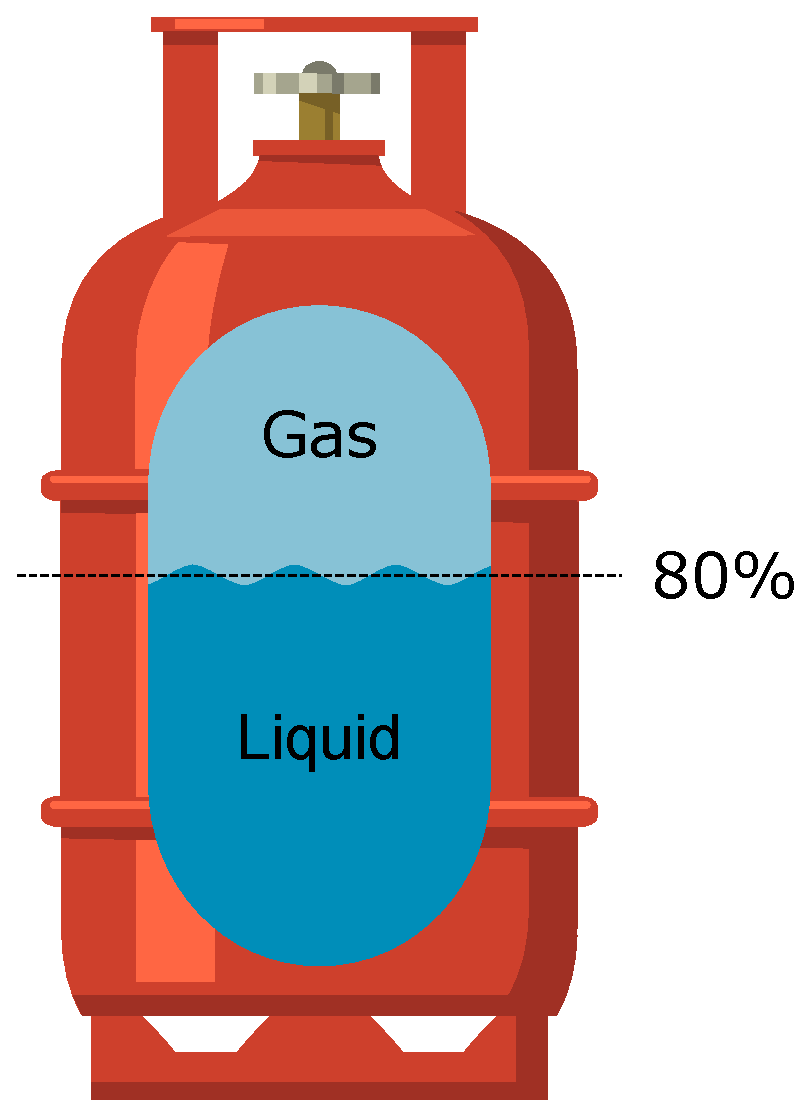
\includegraphics[width=0.25\textwidth]{Chapters/2CHP/Diagrams/bottleBaseliqGas.eps}
    \caption{LPG cylinder internal state composition}{}
    \label{fig:intcomplpg}
\end{figure}

When the cylinders are empty and need to be filled, there is a direct relation between the amount of pressure, needed to fill the cylinders, and the temperature of the gas, the higher the temperature of the gas the higher is the pressure needed to fill the cylinder, this process of turning the LPG in a gas form into a liquid by pressurizing it, is called liquefaction. Another relation that must be taken into consideration, is the weight of the cylinder and the amount of liquid LPG, when the cylinder valve is open and LPG gas is released, the liquid LPG is turns into gas in order to keep a balance of pressure inside the cylinder, since that for the same pressure the density of the LPG liquid is higher then the density of the LPG gas, when the amount of liquid LPG decreases the weight of the cylinder also decreases~\cite{WhatAreProperties,PropaneDensitySpecific}.

%%Correct about gas pressure inside the bottle

%----------------------------------------Section 2-----------------------------------
\section{Measuring/Stimulation Techniques}\label{sec:measStim}
\subsection{Measuring Techniques}
As the LPG cylinder content is divided in two physical states, liquid and gaseous, over the years several techniques have been used and improved in measuring the liquid level, which is how is determined the amount of LPG in the cylinder, some of the different techniques used are based on the same method. Those methods are usually split in two different categories, contact and contactless. Contact measuring methods usually include, mechanical, electrical or pressure sensing devices. In this methods the sensors are in direct contact with the liquid. In contactless, the methods used usually are more complex to process, when compared with contact methods. In this case the methods of measuring are mainly through optical, ultra-sound, vibration and weight analysis~\cite{nakagawaContactlessLiquidLevelMeasurement2013a}. 
\begin{figure}[]
    \centering
    \begin{subfigure}{0.15\textwidth}
        \centering
        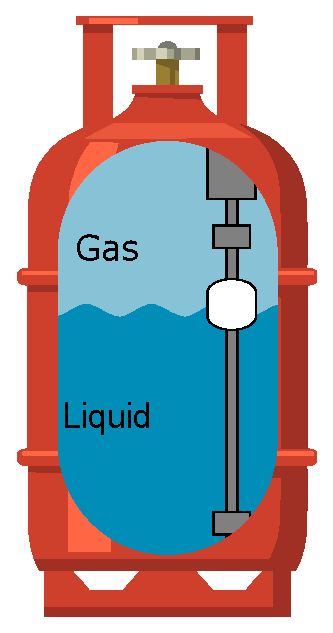
\includegraphics[width=\linewidth]{Chapters/2CHP/Diagrams/bottleBasefluctuator.eps}
        \caption{}{}
        %\label{subfig:g1lines}
    \end{subfigure}
    \begin{subfigure}{0.15\textwidth}
        \centering
        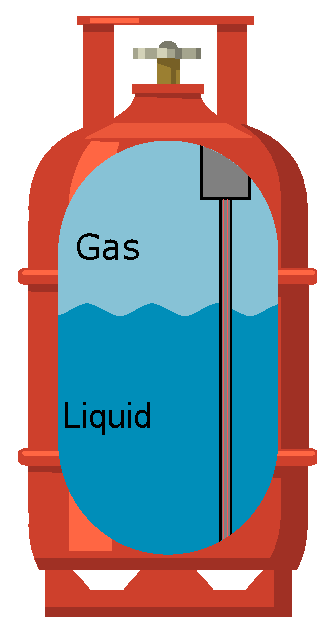
\includegraphics[width=\linewidth]{Chapters/2CHP/Diagrams/bottleBaseelectrode.eps}
        \caption{}{}
        %\label{subfig:g2lines}
    \end{subfigure}
    \begin{subfigure}{0.15\textwidth}
        \centering
        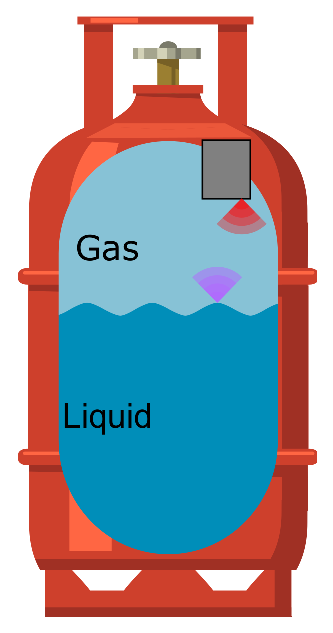
\includegraphics[width=\linewidth]{Chapters/2CHP/Diagrams/bottleBaseultrasound.eps}
        \caption{}{}
        %\label{subfig:g3lines}
    \end{subfigure}
    \begin{subfigure}{0.15\textwidth}
        \centering
        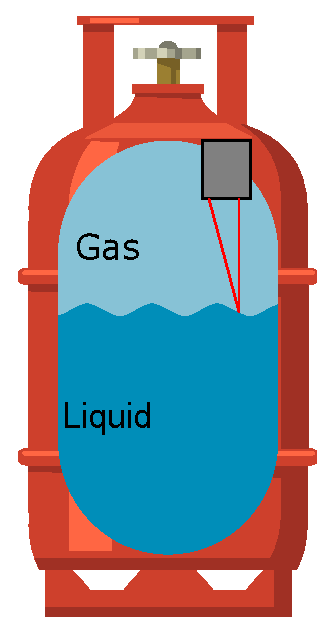
\includegraphics[width=\linewidth]{Chapters/2CHP/Diagrams/bottleBaseoptical.eps}
        \caption{}{}
        %\label{subfig:g4lines}
    \end{subfigure}
    \caption{Different LPG cylinder to used to compare the relation between Frequency and Weight for different models}{~\cite{wuLiquidLevelDetector2014b}}
     %\label{fig:noise}
 \end{figure}
Taking in consideration the fact that a LPG cylinder is opaque and isolated, some of the methods can't be used in the process, for instance, a mechanical float-type isn't a suitable solution to use inside the cylinder, or in the same way to use an electrode, as a electrical method, in these cases the device would require to be installed inside the cylinder during his fabrication process, possibly implying the substitution of the current cylinders. In the same way, in contactless methods, the use of different optical techniques and the use of of ultra-sound, would face the same problem mentioned with the contact methods, being also discard as a suitable method in this situation. 

From previous research, some work has already been developed with the purpose of measuring the amount of liquid gas inside a LPG cylinder. Being the techniques used based on the methods presented above.
%Based on the pressure
In a work from ~\citeauthor{baigAccurateMeasurementPressure2008b} a pressure sensing device was developed, with the final appliance to a LPG cars, but with the possibility of apply in other circumstances. The device uses the pressure variation to move a magnet and using a Hall Effect sensor, with a fixed position, this motion produces a linear change of the voltage in the sensor, giving an accurate method of measuring the amount of gas in the LPG cylinder, in this case~\cite{baigAccurateMeasurementPressure2008b}. 
%Based on the weight
A common method of evaluate the amount of gas inside a LPG cylinder, is based on the weight change of the cylinder, that decreases with the consumption of liquid gas. As an example, the work developed by ~\citeauthor{dasilvamedeirosSmartgasSmartPlatform2017a}, ~\citeauthor{shresthaIoTBasedSmart2019a} or ~\citeauthor{shinganSmartGasCylinder2017a} have similar approaches to measure the amount of liquid gas inside the LPG cylinder. There is various works based on this technique since is very simple to implement and very precise, it only requires a load cell, a amplifier, a microcontroller and a method to display the results, and unless there is a huge change in the external temperature, the density of the gas won't be much affected and thus not affecting the weight of the bottle~\cite{dasilvamedeirosSmartgasSmartPlatform2017a,shresthaIoTBasedSmart2019a,shinganSmartGasCylinder2017a}.
%Based on Wave analysis
Another method, that proved to be valid for measuring the amount of liquid inside a closed opaque container, is based on the analysis of the resulting vibrations when the container is stimulated by a external source. Depending in the type of the stimulation, it can produce only vibration, or it can also produce a characteristic sound, for different levels. As a example of two approaches based on the same principle are the works from ~\citeauthor{jahnLevelSensorFluids2014a} and ~\citeauthor{wuAnalysisImplementationNoncontact2016a}, in both cases the vibrations are analyzed, in one case is the vibration of the tank and in the other is through the sound produced by the tank vibration~\cite{jahnLevelSensorFluids2014a,wuAnalysisImplementationNoncontact2016a}. Since the approach is through the analysis of the vibration, the stimulation methods for this method will be presented ahead. 

\subsection{Stimulation Techniques}
Taking into consideration, that the measurment of the liquid level is based on the vibration, it was found in previous work two techniques to induce the vibration in the LPG bottle.
The first example of a technique of stimulation the LPG bottle is by using a piezoelectric transducer, attached to the bottom of the container, this transducer produces transversal and longitudinal waves in the surface of the container where the transducer is attached. The frequency of the waves generated is related with the frequency of the system response to a certain level, and changes according to that. The same waves are captured with another piezoelectric transducer and processed~\cite{jahnLevelSensorFluids2014a}.
\begin{figure}[]
    \centering
    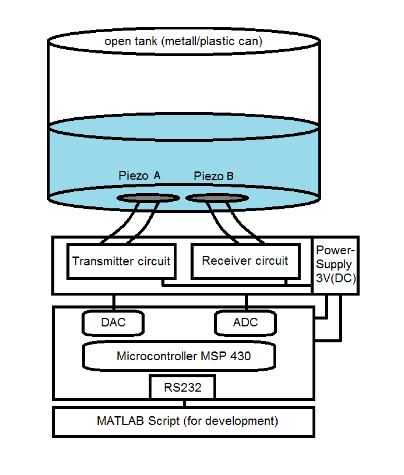
\includegraphics[width=0.35\textwidth]{Chapters/2CHP/Diagrams/stimPiezo.eps}
    \caption{Stimulation and measuring system based on piezo transducer}{~\cite{jahnLevelSensorFluids2014a}}
    \label{fig:stimPiezo}
\end{figure}
Another method to produce vibration in the LPG bottle, can be archived with a hammer or a device, that hits the surface of the LPG bottle, the captured signal is the appropriated sensor is then processed and the result returns the level of liquid gas inside. In this case, not only vibration in the bottle is produced but a sound as well~\cite{wuAnalysisImplementationNoncontact2016a}.
\begin{figure}[]
    \centering
    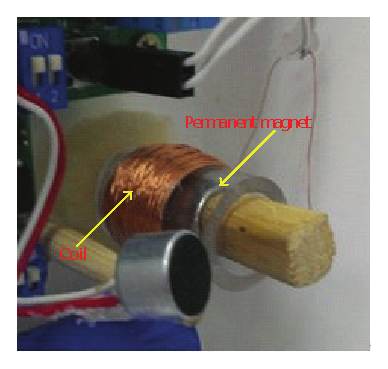
\includegraphics[width=0.45\textwidth]{Chapters/2CHP/Diagrams/stimHammer.eps}
    \caption{Stimulation system based on a knocking device}{~\cite{wuAnalysisImplementationNoncontact2016a}}
    \label{fig:stimHammer}
\end{figure}

%----------------------------------------Section 3-----------------------------------

\section{Signals and System}\label{sec:sigNsys}
\subsection{Vibration}
The vibration and the studies in this field are usually related with the oscillatory motion of a body and the forces associated with them. Bodies with mass and elasticity are capable of experience vibration, knowing that, for example, when a structure is design, is required to take in consideration the oscillatory behavior of the structure. There are two types of vibration, free and forced. The first takes place when a system oscillates under forces natural to the system itself and there is no action of external forces. Under free vibration the system will vibrate at one or more of its natural frequencies, stablished by the properties of the system. Forced vibration occurs when the system is under the excitation of external forces. If it oscillatory, the system will vibrate at the same frequency of the external oscillation, if this frequency matches one of its natural frequencies a resonant state is reached, which may dangerous for a structure stability.   

\subsection{Signal definition}
Signals can describe a large variety of physical phenomenon's, bringing a certain information about it, depending of the phenomenon represented. For example, the voltage variation in a capacitor, or the human voice which creates variations in acoustic pressure, captured by a microphone that senses those variations and convert them into a electrical signal. A signal can be represented mathematically as a function of one or more independent variables. 
To what concern in signal processing, the types of signal considered are two types, continuous-time signals and discrete-time signals. In these cases, the independent variable is continuous and discrete, respectively~\cite{oppenheimSignalsSystems1997}.

\subsection{Signal and Digitalization}
A continuous-time signal can be represented in a discrete-time form by the knowledge of its values at certain points in time equally spaced. This is called sampling theorem, and if the samples are close to each other, less time between samples, the more similar the discrete signal became to the continuous. Sampling plays an important role between the continuous-time and the discrete-time.

Considering a continuous-time signal $x(t)$ is measured at every $T_{s}$ seconds. The is discretized in units of the sampling interval $T_{s}$:
\begin{figure}[]
    \centering
    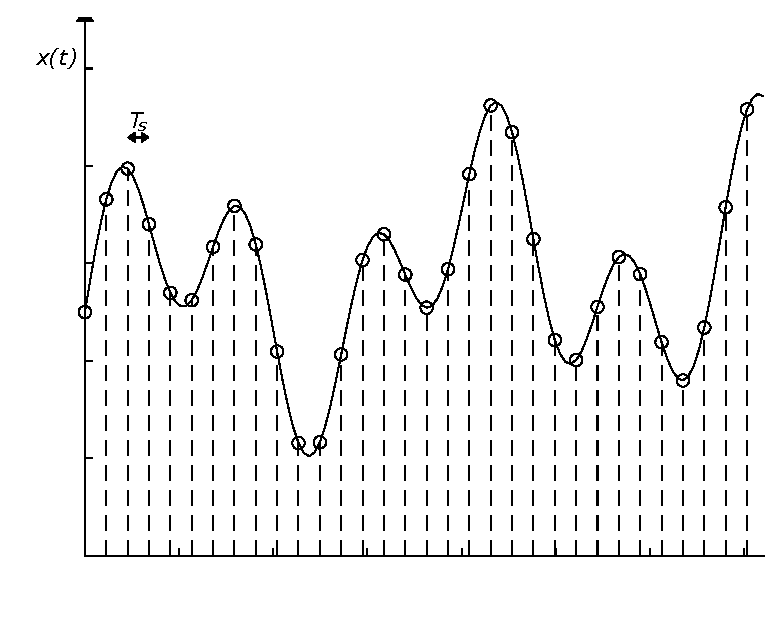
\includegraphics[width=0.45\textwidth]{Chapters/2CHP/Diagrams/sampsignal.eps}
    \caption{Signal sampling}{}
    \label{fig:signalsamp}
\end{figure}
\begin{center}
    $t = nT_s,\> n = 0, 1, 2, ...$
\end{center}
The variable $T_s$ is called sampling period and the inverse of the period $f_s=\frac{1}{T_s}$ being the sampling frequency. One of the problems of this conversion is usually related with the correct choose of the sampling period, for that the theorem clearly specifies that the sampling period must be small enough so if there are small variations in the signal, they don't get lost between samples. Therefor the theorem says that the sampling frequency $f_s$ must be chosen to be  at least twice the maximum frequency $f_{max}$. A continuous-time signal $x(t)$ is bandlimited, so its frequency spectrum is limited at maximum frequency $f_{max}$, and no frequencies above that.

\begin{equation} \label{eq:sampFreq}
       f_s \geq 2f_{max}
\end{equation}
\begin{equation} \label{eq:sampPeriod}
    T_s \leq \frac{1}{2f_{max}}
\end{equation}

The minimum value of the sampling frequency allowed by the theorem, is called the Nyquist rate, and his value is $f_s = 2f_{max}$. Oppositely, for a known value of $f_s$ the maximum frequency of the signal is $f_{max}=\frac{f_s}{2}$ and is called the Nyquist frequency of folding frequency.

For the representation of some signals is usually used a unit impulse as a method to build a block to represent and construct other signals. The simplest representation of a unit impulse (or unit sample), in discrete-time, is defined as follows:
\begin{equation}
    \delta(n) = \left\{ \begin{matrix} 
    0, n \ne 0\\
    1, n = 0\\
    \end{matrix}\right.
\end{equation}
Another example of a simple discrete-time signal is the unit step, defined as:
\begin{equation}
    u(n) = \left\{ \begin{matrix} 
    0, n < 0\\
    1, n \geq 0\\
    \end{matrix}\right.
\end{equation}
If a close analysis is made, is possible to conclude that there is a relation between a unit impulse and a unit step, a unit step can be represented as a sum of impulses
\begin{equation}\label{eq:step}
    u(n) = \sum_{k=0}^{\infty}\delta(n-k)
\end{equation}
The equation \ref{eq:step} can be seen as a sum of delayed impulses and plays an important role in the sampling property.

The values of the $f_{max}$ and $f_s$ depend on the application, and the Nyquist frequency usually defines the cutoff frequencies used in filters required in DSP applications. A example of the of the typical sampling rates of common DSP applications are shown in the following table:   
\begin{table}[]
   \centering
   \begin{tabular}{|c|c|c|} \toprule
       {application}&{$f_max$}&{$f_s$}\\
       \toprule
       {geophysical}&{500 Hz}&{1 kHz}\\
       {biomedical}&{1 kHz}&{2 kHz}\\
       {mechanical}&{2 kHz}&{4 kHz}\\
       {speech}&{4 kHz}&{8 kHz}\\
       {audio}&{20 kHz}&{40 kHz}\\
       {video}&{4 MHz}&{8MHz}\\
       \bottomrule
   \end{tabular} 
   \caption{Common sampling rates per application}{~\cite{orfanidisIntroductionSignalProcessing1996}}  
    \label{tab:sampRat}     
\end{table} 

\subsection{System definition}\label{subsec:SysDef}
There is no specific nature to a system, and there is vast example of systems all around us, they could be biological, mechanical, electrical, among others. In the signal processing context a system can be viewed as a process in which input signals are transformed by the system or cause the system to respond in some way, with the resulting in new output signals. Simplifying, a system can be described as an entity with a specific function, where the output signal is the result of the manipulation one or more input signals.
To the types of signals mentioned, continuous and discrete, the systems usually are represented as in the equation \ref{eq:systemeq}, in both cases $x$ represents input and $y$ output.
\begin{figure}[]
    \centering
    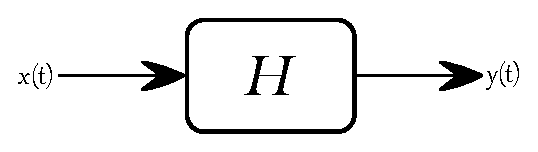
\includegraphics[width=0.45\textwidth]{Chapters/2CHP/Diagrams/systemIll.eps}
    \caption{Generic system}{}    
    \label{fig:systemIll}
\end{figure}
\begin{equation} \label{eq:systemeq}
    \begin{split}
        y(t) = H[x(t)] \\
        y(n) = H[x(n)]
    \end{split}
\end{equation}

One of the motivations for the study/analysis of systems from various applications, thus systems from different applications, with similar behavior, can have similar mathematical descriptions. The description of a system as a mathematical function also allows to simulate the behavior in a certain application, testing the response of it with different techniques. 

A system can be described with certain properties, each one having a different effect on the system output. The properties are stability, memory, causality, invertibility, time-invariance and linearity. In signal-processing context, invertibility and time-invariance have special relevance, with a profound study of linear time-invariant(LTI) systems further ahead~\cite{oppenheimSignalsSystems1997,haykin1999signals}.
\subsubsection*{Stability}
A system is considered stable if an input signal limited in amplitude, results in a output signal also limited in amplitude. The system operation, H, is stable if the output signal $y(t)$  satisfies the following condition
\begin{equation}
    |y(t)|\leq M_y < \infty , \forall t
\end{equation}
If the input signal $x(t)$ satisfies the condition
\begin{equation}
    |x(t)|\leq M_x < \infty , \forall t
\end{equation}
The values of $M_x$ and $M_y$ correspond to finite positive numbers. The conditions for the stability of a discrete-time system can be described in the same way.
\subsubsection*{Memory}
A system has memory, when the output signal depends on past values of the input signal. The temporal extension of the past values on which the output depends, defines how far the memory of the system extends. One example of a system with memory is the current $i(t)$ in a inductor and the relation of his voltage $v(t)$:
\begin{equation}
    i(t)=\frac{1}{L}\int_{-\infty}{t}v(\tau)d\tau
\end{equation}
For a discrete-time system, the conditions are similar. 
\subsubsection*{Causality}
A system is considered \textit{causal} if his resulting output signal, only depends in present/past values of the input signal. Opposed to that, a \textit{noncausal} system can have is output depending on future values of the input signal.
An example of a \textit{causal} output is the following:
\begin{equation}
    y(n) = \frac{1}{3}(x(n)+x(n-1)+x(n-2))
\end{equation}
On the other hand an example of a \textit{noncausal} is:
\begin{equation}
    y(n) = \frac{1}{3}(x(n+1)+x(n)+x(n-1))
\end{equation}
\subsubsection*{Invertibility}
A system is considered invertible if is possible to recover the input from the output signal of the system. The operation to recover the signal may be a different system connected to the output of the first. If the operation of a system is represented with $H$ in a continuous-time domain, with $x(t)$ and $y(t)$ being the input and output, respectively. The $y(t)$ is applied to the second system, where the result is expected to be $x(t)$, as follows:
\begin{equation}
    \begin{aligned}
        H^{-1}{y(t)} = H^{-1}{H\{x(t)\}}\\
        = H^{-1}H\{x(t)\}    
    \end{aligned}
\end{equation} 
As the $H^{-1}H$ denotes the identity operation. If $H^{-1}$ is the inverse operation of the $H$ then the output of the second operation is the same as the input of the first operation. This property has special relevance in the design of communications systems. 

\subsubsection*{Time-Invariance}
A system is considered time invariant if a time delay in the input signal, results as well in a delay of the output signal. This means that a certain system will respond in the same way, whenever a signal is applied in input, meaning that the characteristics of the system won't change with time. Considering a continuous-time system, with $x(t)$ and $y(t)$ being the input and the output, respectively. Represented as follows:
\begin{equation}
    y(t) = H\{x(t)\}
\end{equation} 
If the input signal is delayed by $t_0$ seconds, the new input signal is $x(t-t_0)$ and an be described as follows:
\begin{equation}
    x(t-t_0) = S^{t_0}\{x(t)\}
\end{equation}
Where the $S^{t_0}$ represents the delay. So the new output signal $y_i(t)$, resulting from the delay applied in the will be:
\begin{equation}
    \begin{aligned}
        y_i(t) = H\{x(t-t_0)\}\\
        = H\{S^{t_0}\{x(t)\}\}\\
        =HS^{t_0}\{x(t)\}    
    \end{aligned}
\end{equation}
Now considering $y_o$ the output signal of the original system delayed by $t_0$ seconds: 
\begin{equation}
    \begin{aligned}
        y_i(t) = S^{t_0}\{y(t)\}\\
        = S^{t_0}\{H\{x(t)\}\}\\
        =S^{t_0}H\{x(t)\}    
    \end{aligned}
\end{equation}
The system is time invariant if the outputs are equal for an identical input signal $x(t)$. 
\begin{equation}
    HS^{t_0} = S^{t_0}H
\end{equation}
This means that, for a system $H$ to be time invariant, the system $H$ and the time delay $S^{t_0}$ must commute with each other for $t_0$. A similar relation in the discrete-time system to be time invariant.  
\subsubsection*{Linearity}
A system is considered \textit{linear} if fills all the requirements of the \textit{principle of superposition}. That is, if the response of a system to a weighted sum of input signals is equal to the same weighted sum of the output signals, in each one of the output signals being the result of a certain input signal acting independently in the system. If this principle is not fulfilled, the system is called \textit{nonlinear}. 
A weighted sum of continuous-time signals: 
\begin{equation}
    x(t) = \sum_{i=1}^{N}a_ix_i(t)
\end{equation}
Is applied to a system $H$, where $a_1, a_2, ..., a_N$ correspond the weight factor and $x_1(t), x_2(t), ..., x_N(t)$ correspond to the input signals. Resulting in the system response as represented:
\begin{equation}
    \begin{aligned}
        y(t) = H\{x(t)\}\\
        =H\Bigg\{\sum_{i=1}^{N}a_ix_i(t)\Bigg\}\\
    \end{aligned}
\end{equation} 
If the system is linear then, the weighted sum of output signals is:
\begin{equation}
    \begin{aligned}
        y(t) = \sum_{i=1}^{N}a_i y_i(t)\\
        y_i(t) = H\{x_i(t)\}   
    \end{aligned}
\end{equation}
This result in
\begin{equation}
    y(t) = \sum_{i=1}^{N}a_i H\{x_i(t)\}    
\end{equation}
which is the equivalent mathematical representation as in a weighted sum of inputs. To represent them in the same form, the system operation can commute with the amplitude and sum scaling. This principle also applies to discrete-time systems in a similar form. 


\subsection{LTI Systems} \label{subsec:LTI}
As systems can be found all around us, so does a LPG bottle can be considered as a system. If the mathematical model that represents it meet the last two properties mentioned, it can be referred as a linear time-invariance (LTI) system. These properties combined with the characteristics of the unit impulse, being able to represent common signals as a representation of combined delayed impulses, this allows to completely characterize a LTI to what referrers his impulse response~\cite{oppenheimSignalsSystems1997,haykin1999signals}.
Similar to a unit step $u(n)$, a common signal $x(n)$ can be represented by unit impulses, as follows:
\begin{equation}
    x(n) = \sum_{k=-\infty}^{+\infty} x(k)\delta(n-k)
\end{equation}
In this case the weights in the linear combination are $x(k)$. Another aspect to take in consideration in these types of systems, is the response of the system to a impulse $\delta(n)$, results in $h(n) = H[\delta(n)]$. With this in mind, the response of a linear system $y(n)$ to a common input signal $x(n)$, represented from a combination of shifted impulse, can be represented as:
\begin{equation}
    \begin{matrix}
        y(n) & = & H\big[x(n)\big] \\
        \ & = & \sum_{k=-\infty}^{+\infty} x(k)h(n-k)
    \end{matrix}
\end{equation}
The result is known as the \textit{convolution sum} or \textit{superposition sum} and the operation as \textit{convolution} of the sequences $x(n)$ and $h(n)$. The operation can be represented as:
\begin{equation}
    y(n) = x(n) * h(n)
\end{equation} 
\subsection{Discrete-Time Fourier-Transform}
For the analysis of LTI systems, one of the most powerful and used tools is the Fourier-Series and Fourier Transform. For the analysis purpose, the focus is only going to be the Discrete-Time Fourier-Transform (DTFT). The study of this type of systems offers two great advantages:
\begin{itemize}
    \item It is possible to construct a extensive and convenient class of signals, based on a set of simpler signals.
    \item The response of the LTI signal should be simple enough, to provide a convenient representation of the response from the system to any signal based on the combination of several other basic signals. 
\end{itemize} 
The properties are provided by a set of exponential signals, this is important because the response of a LTI system to a complex exponential input, is the same exponential with the change in amplitude. When dealing with complex exponential signals, for the domain of analysis changes, which is in this case the frequency domain.

For the analysis purpose, is necessary to know the representation of a signal $x(n)$, that later is going to be represented as a input of a system. The signal is represented in the frequency domain, where $\omega$ represents the \textit{angular frequency}, and its period is $2\pi$. The signal is represented as follows:
\begin{equation}
    X(e^{\jmath \omega})=\sum_{n=-\infty}^{+\infty}x(n)e^{-\jmath \omega n}
\end{equation}
As mentioned in \ref{subsec:LTI}, the response of a LTI system to a impulse, can be represented by the \textit{convolution} operation. This operation can be represented in the frequency domain as:
\begin{equation}
    Y(e^{\jmath\omega})= X(e^{\jmath\omega})H(e^{\jmath\omega})
\end{equation}
Where the terms $X(e^{\jmath\omega})$, $H(e^{\jmath\omega})$ and $Y(e^{\jmath\omega})$ are the Fourier transforms of $x(n)$, $h(n)$ and $y(n)$, respectively. The \textit{convolution} operation in the LTI system, is easily represented using the Fourier transform with a simple algebraic operation, by multiplying the Fourier transforms. This facilitates the analysis of the signals and systems and increases the understanding in the behavior of the LTI system when a signal is applied to its input.

With this work in consideration, a algorithm was presented by Cooley and Tukey, the fast Fourier Transform, or simply FFT. This algorithm later proved to be suitable for a digital implementation, with its reducing time in computing the transforms by order of magnitude~\cite{oppenheimSignalsSystems1997}.



% ---------------------------------------Section 4-------------------------------------------------
\section{LPG cylinder Model}\label{sec:LPGModel}
As already mentioned \ref{subsec:SysDef}, is possible to describe an LPG cylinder over a mathematical function, as a system. Being, in many cases, the description similar to other systems. The fact that the system is described as a mathematical model allows to understand what it could be the behavior of it. 

The work developed by \citeauthor{wuLiquidLevelDetector2014b} proposes a model for the LPG cylinder, based on acoustic principals to perform measurements. The procedure that they implement is quite simple, by knocking on the side of the cylinder, that generates the sound, usually that sound changes according to the amount of liquid inside of the cylinder, to evaluate what is the amount of gas inside, the vibration in the cylinder wall is recorded and the frequency of the sound give is proportional to the amount of gas present inside.

Before them, other researches were conducted to study the transverse vibration of cylindrical tubes with variable levels of liquid inside. One of them is the work of \citeauthor{chanFreeVibrationCantilever1995} who proposed a vibration model (clamped-free model), where a tube, clamped at bottom and free at top, was used to study the relations resonant frequencies versus liquid levels. Their tests were conducted under a controlled environment, for different levels of liquid, and the experimental results obtained were in accordance with the theoretical calculations~\cite{chanFreeVibrationCantilever1995}.

Their work was then extended with a different approach by \citeauthor{chanFREEVIBRATIONSIMPLY1996}, the model they proposed study the vibration of a simply supported beam with uniform mass, partially loaded, in one of the sides, with a distributed mass(pinned-pinned model). For the conducted tests, the load length added increases until reaching the the length of the beam, the results obtained in their measurements agreed with the results obtained from the previous work\cite{chanFREEVIBRATIONSIMPLY1996}. 
A few years later \citeauthor{jacobsContactlessLiquidDetection2005} proposed a similar model to \citeauthor{chanFreeVibrationCantilever1995} model, but this time with different boundaries, clamped at bottom and top (clamped-clamped model). The tests conducted measure the resonant frequency of the tube, for different levels of liquid, and their results fitted with the results obtained in the previous mentioned tests~\cite{jacobsContactlessLiquidDetection2005}.

Like in the previous studies, the base of the work developed by \citeauthor{wuLiquidLevelDetector2014b} is the Euler-Bernoulli beam theory\cite{raoMechanicalVibrations2017,thomsonTheoryVibrationApplications1996}, this is used to create a model of a cylindrical tube, allowing to estimate the vibration frequencies for different liquid levels. In their work they were able to prove that this theory can be applied to the vibrations in a LPG cylinder, where the results obtain similar to the results obtained in previous works, also based in the same principal.

\subsection{Mathematical Model for LPG cylinder}
The similarities with the Euler-Bernoulli theory and its models, with a LPG cylinder, is related with the construction of the cylinder. A common LPG cylinder used in house appliances has two welded seams, located at the bottom and the top, and those seams are considered the boundaries of the LPG. These boundaries are not considered to be free, but loose instead, with doesn't allow to immediately conclude which type of the mentioned boundaries the cylinder has. Before getting into a conclusion is necessary to understand the theory behind their work.

If a hammer is used to knock the lateral surface of the LPG cylinder, this will trigger a transverse vibration, considered in this case a mechanical vibration. This vibration is similar to Euler-Bernoulli beam, assuming a distributed mass per unit of length $m$, partially loaded with a distributed mass as well $m_d$, corresponding in this situation to the liquid part of the cylinder. In \ref{fig:mechanicalmodel} is identified the boundaries and is illustrated the LPG cylinder model, the  equation \ref{eq:beamEqSimp} describe the vibratory model of the LPG cylinder. The liquid-gas interface corresponds to the origin, and $EI$ is a constant value corresponding to the the beam flexural rigidity
%Mechanical model of the LPG bottle
\begin{figure}[]
    \centering
    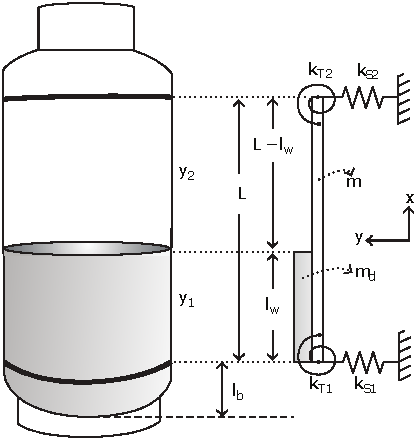
\includegraphics[width=0.45\textwidth]{Chapters/2CHP/Diagrams/mathmodelLPG.pdf}
    \caption{The LPG cylinder filled with liquid, with the mechanical representation of the Euler-Bernoulli beam}{\cite{wuLiquidLevelDetector2014b}}
    \label{fig:mechanicalmodel}
\end{figure}
\begin{equation} \label{eq:beamEqSimp}
    \begin{split}
        EI\frac{\partial^4y_1}{\partial x^4} + (m + m_d)\frac{\partial^2y_1}{\partial t^2} = 0,\> & \text{for $-l_w \leq x < 0$} \\
        EI\frac{\partial^4y_2}{\partial x^4} + m\frac{\partial^2y_2}{\partial t^2} = 0,\> & \text{for $0 < x < L-l_w$}
    \end{split}
\end{equation}

The variables $y_1$ and $y_2$ correspond to the transverse vibratory displacements o f the beam. Considering that the seam welding's are not ideally clamped or pinned, and the main transverse vibration is restricted between the two boundaries, is assumed that they have small displacements, that will show flexural vibration. This way their model assumes that there is strong linear springs and torsional springs connected at the boundaries. Which obligates to the boundaries conditions to be formulated taking in consideration these factors, where $k_{S1}$, $k_{T1}$ are the linear and torsional springs constants for the lower welding, and $k_{S2}$, $k_{T2}$ are the correspondent spring constants in the upper welding.
\begin{equation} \label{eq:beamEqEv}
    \begin{split}
        At\>x=-l_w \Rightarrow \begin{cases}
            EI\frac{\partial^2y_1}{\partial x^2} = -k_{T1}\frac{\partial y_1(-l_w,t)}{\partial x}\\
            EI\frac{\partial^3y_1(-l_w,t)}{\partial x^3}=-k_{S1}.y_1    
        \end{cases}\\
        At\>x=L-l_w \Rightarrow \begin{cases}
            EI\frac{\partial^2y_2}{\partial x^2} = -k_{T2}\frac{\partial y_2(L-l_w,t)}{\partial x}\\
            EI\frac{\partial^3y_2(L-l_w,t)}{\partial x^3}=-k_{S2}.y_2    
        \end{cases}    
    \end{split}
\end{equation}

At the bottom a circular steel plate is attached to make the cylinder more stable in relation with the ground, this turns it more stable the the upper part, which allow them to conclude that the value of the constants, linear and torsional springs, of the bottom is higher when compared with the upper values, i.e. $k_{S1}>k_{S2}$ and $k_{T1}>k_{T2}$. The continuity and equilibrium condition at the interface of the liquid, inside the cylinder, are:
\begin{equation} \label{eq:beamEqEquilCond}
    \begin{split}
        y_1(0,t) = y_2(0,t),\> y'_1(0,t) = y'_2(0,t) \\
        y''_1(0,t) = y''_2(0,t),\> y'''_1(0,t) = y'''_2(0,t)
    \end{split}
\end{equation}
This conditions allow them to investigate the relation of the normalized frequency ratio $f_r=f/f_0$, considering $f_0$ as the maximum frequency when there is no liquid inside, and the length ratio $l_w/L$ in their experiments.

\subsection{Relation with previous studies}
So far the model presented show very general boundaries conditions, by controlling the variables, the model can be easily compared with the mentioned model. Taking that into consideration, a demonstration of this similarities was presented and is the following.
    \subsubsection{Clamped-free boundaries}
    For this condition, the values of the variables are considered to be $k_{S1}=k_{T1}\approx\infty$ and $k_{S2}=k_{T2}=0$. When \citeauthor{chanFreeVibrationCantilever1995} proposed this model to calculate the frequencies of a cantilever tube, partially filled with liquid mercury, the cantilever was clamped at the bottom and free at the top, and the transverse vibration was generated by using a hammer to knock the tube\ref{fig:clampedfreemodel}. 
    %clamped-free model
    \begin{figure}[]
        \centering
        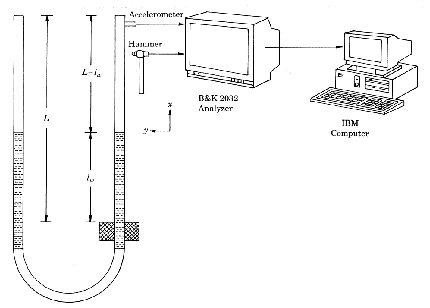
\includegraphics[width=0.45\textwidth]{Chapters/2CHP/Diagrams/clampedfreemodel.pdf}
        \caption{Clamped-Free Model}{~\cite{chanFreeVibrationCantilever1995}}
        \label{fig:clampedfreemodel}
    \end{figure}
    If the values of the variables are replaced in the equation\ref{eq:beamEqSimp} the result of this setup makes the boundaries conditions at their limits, $x=-l_w$ and $x=L-l_w$, to be as shown in \ref{eq:beamEqClamFree}, when comparing the results in the boundaries conditions they verify that they were the same as in~\cite{chanFreeVibrationCantilever1995}.
    \begin{equation} \label{eq:beamEqClamFree}
            y_1(-l_w,t) = y'_1(-l_w,t) = y''_2(L-l_w,t) = y'''_2(L-l_w,t)=0
    \end{equation}
    \subsubsection{Pinned-pinned boundaries}
    For this condition, the value of the variables considered is $k_{S1}=k_{S2}\approx\infty$ and $k_{T1}=k_{T2}=0$. In this model, proposed by \citeauthor{chanFREEVIBRATIONSIMPLY1996}, the study is made in a simply supported beam partially load, with distributed mass in both cases\ref{fig:pinnedpinnedmodel}.
    %Pinned-Pinned Model
    \begin{figure}[]
        \centering
        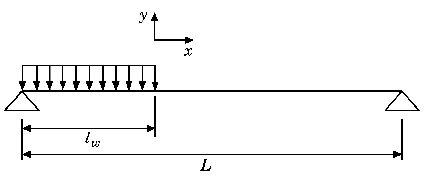
\includegraphics[width=0.45\textwidth]{Chapters/2CHP/Diagrams/pinnedpinnedmodel.pdf}
        \caption{Pinned-Pinned Model}{~\cite{chanFREEVIBRATIONSIMPLY1996}}
        \label{fig:pinnedpinnedmodel}
    \end{figure}
    Once again, if the variables in \ref{eq:beamEqSimp} are replaced with $k_{S1}$, $k_{T1}$, $k_{S2}$ and $k_{T2}$, the result in this setup will also match the boundaries condition\ref{eq:beamEqPinnedx2} at $x=-l_w$ and $x=L-l_w$, obtained in \cite{chanFREEVIBRATIONSIMPLY1996}.
    \begin{equation} \label{eq:beamEqPinnedx2}
        y_1(-l_w,t) = y''_1(-l_w,t) = y_2(L-l_w,t) = y''_2(L-l_w,t)=0
    \end{equation}
    \subsubsection{Clamped-clamped boundaries}
    In this case, the value considered to the variables was $k_{S1}=k_{T1}=k_{S2}=k_{T2}\approx\infty$. This model, proposed by \citeauthor{jacobsContactlessLiquidDetection2005}, with a contactless method to measure the vibration of a opaque capillary tube\ref{fig:clampedclampedmodel}.
    %Clamped-Clamped Model
    \begin{figure}[]
        \centering
        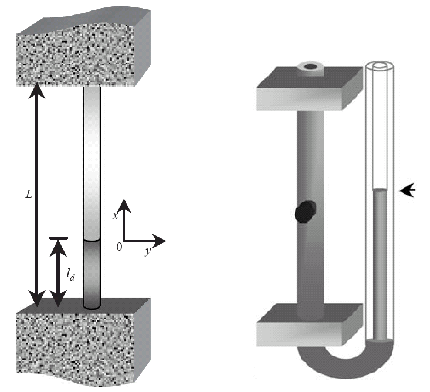
\includegraphics[width=0.45\textwidth]{Chapters/2CHP/Diagrams/clampedclampedmodel1.pdf}
        \caption{Clamped-Clamped Model}{~\cite{jacobsContactlessLiquidDetection2005}}
        \label{fig:clampedclampedmodel}
    \end{figure}
    Following the same path of the previous two, the variables $k_{S1}$, $k_{T1}$, $k_{S2}$ and $k_{T2}$ were once again replaced in \ref{eq:beamEqSimp},and the results obtained\ref{eq:beamEqClampedx2} at their boundaries conditions matched results obtained in~\cite{jacobsContactlessLiquidDetection2005}
    \begin{equation} \label{eq:beamEqClampedx2}
        y_1(-l_w,t) = y'_1(-l_w,t) = y_2(L-l_w,t) = y'_2(L-l_w,t)=0
    \end{equation}

    \subsubsection{Relation of Frequency versus Length}
    As a final comparison, the test between the relation of the frequency with the length of the liquid level was executed. For that, different values were attributed to linear and torsional spring variables, to allow the simulation of theoretical curves of the normalized frequency ratio $f_r (f_i/f_0)$ and length ratio $l_r (l_w/L)$. The values for each of the variables were chosen to be large enough to simulate the different boundaries conditions. As expected the results[reference to all images] of \citeauthor{wuLiquidLevelDetector2014b} were very similar with what was previously obtained~\cite{chanFreeVibrationCantilever1995,chanFREEVIBRATIONSIMPLY1996,jacobsContactlessLiquidDetection2005}, confirming what was mention in the beginning of this section.
    %Theoretical curves
    \begin{figure}[]
        \centering
        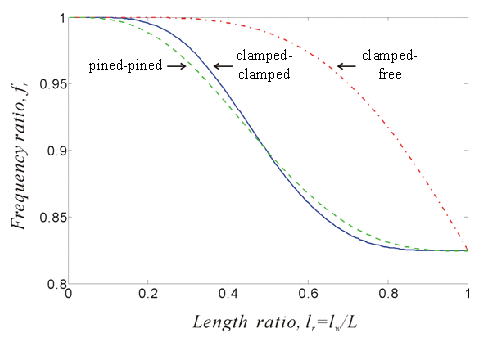
\includegraphics[width=0.45\textwidth]{Chapters/2CHP/Diagrams/theoricalcurve.pdf}
        \caption{Frequency VS Weight - Practical curve obtained by \citeauthor{wuLiquidLevelDetector2014b}}
        \label{fig:theoCurves}
    \end{figure}
    In this relation is important to note that, when the cylinder is almost empty $l_r = 0$ the frequency of the vibration is the highest, in the opposite cases, when the cylinder is full $l_r = 1$ then the vibration frequency is archives the minimum value. 
\subsection{Experimental results}\label{subsec:SOAExpRes}
In the tests perform by \citeauthor{wuLiquidLevelDetector2014b}, their setup consisted in a hammer knocking in the lateral surface of the cylinder, that produces the transversal vibration, which is captured by a microphone,processed with a FFT algorithm. By continuously releasing gas and measure the produced vibration, and the correspondent frequency they obtained the following relation: 
%Practical curve obtained
\begin{figure}[]
    \centering
    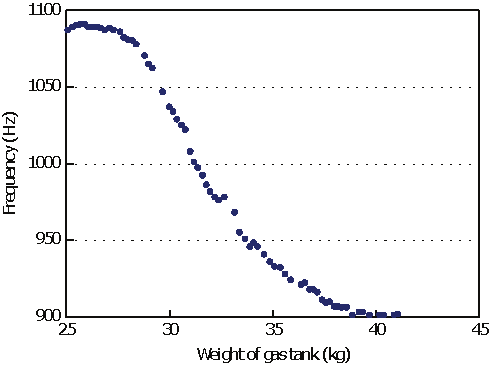
\includegraphics[width=0.45\textwidth]{Chapters/2CHP/Diagrams/weightvsfrequency.pdf}
    \caption{Frequency VS Weight - Practical curve obtained by \citeauthor{wuLiquidLevelDetector2014b}}
    \label{fig:practCurve}
\end{figure}
In the same way of their theoretical simulations, the relation between the vibration frequency and the liquid level(or the length of the liquid) is similar, the highest frequency correspond to the lowest liquid level, and the lowest frequency to the highest liquid level. One thing that is important to refer that is mentioned in their work is, this relation is constant for the different variety of LPG cylinders, but the frequency range of each also varies with the amount of gas that they can store\ref{fig:practCurve}, which means that the device must be adapted to the type of cylinder that is going to be used in. 
%Figures of curves from different bottles
\begin{figure}[]
    \centering
    \begin{subfigure}{0.45\textwidth}
        \centering
        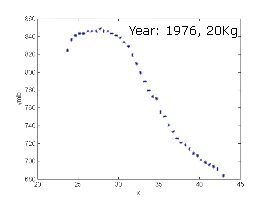
\includegraphics[width=\linewidth]{Chapters/2CHP/Diagrams/g1line.pdf}
        \caption{}
        \label{subfig:g1lines}
    \end{subfigure}
    \begin{subfigure}{0.45\textwidth}
        \centering
        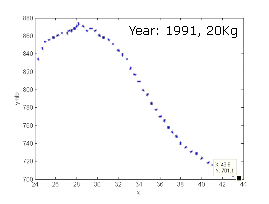
\includegraphics[width=\linewidth]{Chapters/2CHP/Diagrams/g2line.pdf}
        \caption{}
        \label{subfig:g2lines}
    \end{subfigure}
    \begin{subfigure}{0.45\textwidth}
        \centering
        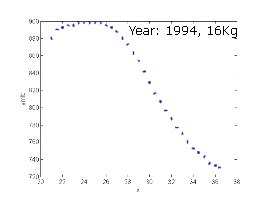
\includegraphics[width=\linewidth]{Chapters/2CHP/Diagrams/g3line.pdf}
        \caption{}
        \label{subfig:g3lines}
    \end{subfigure}
    \begin{subfigure}{0.45\textwidth}
        \centering
        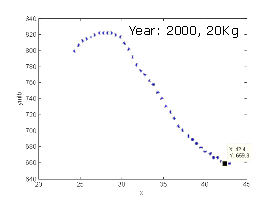
\includegraphics[width=\linewidth]{Chapters/2CHP/Diagrams/g4line.pdf}
        \caption{}
        \label{subfig:g4lines}
    \end{subfigure}
    \caption{Different LPG cylinder to used to compare the relation between Frequency and Weight for different models}{~\citeauthor{wuLiquidLevelDetector2014b}}
     \label{fig:noise}
 \end{figure}
A couple of years latter this work was followed by ~\citeauthor{wuAnalysisImplementationNoncontact2016a}, were they developed a prototype with the function of measure the frequency of the vibration, and thus the returning the liquid level of the LPG cylinder. The setup used and the test conditions were very similar the the previous work.

\section{Vibration Sensors}\label{sec:VibSens}
To acquire and measure the vibration, the sensors used must work according to the system mechanical or optical principals of vibration. There is a large variety of sensors that ca be used for that purpose, although there isn't a direct method, or sensor, to measure the vibration, they can be either mechanical or optical. The sensors can be divided in different groups, based on their behavior, they can be active or passive, the type of measurement can be either absolute or relative, and there is also some specific characteristics of the signals that differ from the type of sensor, like the frequency range, signal dynamic and the quality of the data acquired. Finally sensors are also divided in contact and non-contact measurement and subdivided in path/displacement, speed/velocity or acceleration.

For contact measurements, sensors related to path/displacement can be potentiometric transmitters or Linear Variable Differential Transmitter (LVDT), to speed/velocity it can be applied the principle of electrodynamics or use a seismometer as a sensor and for acceleration the sensors can be piezoelectric, piezo-resistive, resistive or inductive. In non-contact measurements, path/displacement sensors are eddy current sensors, optical sensors and hall sensors, or can be based on the capacitive principle, for speed/velocity is used a Laser-Doppler vibrometer (LDV) and for acceleration isn't possible to measure directly, although it can be derivate from speed/velocity measurement, but induces a lot of noise in the data acquired\cite{SensorsVibrationMeasurement,VibrationMeasurementVibration2019}.

To measure the vibration, usually is the contact acceleration the most common method to measure them, beside the sensors mentioned, is used as well accelerometers, this devices are used in industry to reliably measure vibration in equipment, to monitoring their health.The functioning  principles of accelerometers can differ from one to another. The basic principle of a accelerometer is similar to a seismometer, from this there are 3 main types, mechanical, capacitive and piezoelectric. The mechanical is the most similar to a seismometer, with a mass attached to a spring, every time that acceleration occurs, just like in seismometer, the mass moves and a pen attached to the mass traces the vibration captured.
\begin{figure}[]
    \centering
    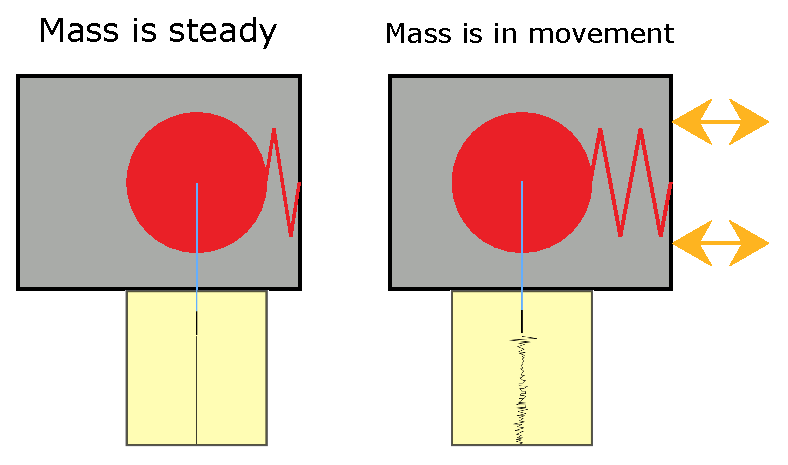
\includegraphics[width=0.45\textwidth]{Chapters/2CHP/Diagrams/seismometer.eps}
    \caption{Illustration of the working principle of simple accelerometer}{}    
    \label{fig:wseismometer}
\end{figure}
%%Insert here a image to illustrate this
% see in https://www.explainthatstuff.com/accelerometers.html  
Although in the case of the accelerometer, doesn't trace with a pen in paper, instead generates a electrical or magnetic signal. A example of this, is a piezoresistive accelerometer, which has a his mass attached to a potentiometer, and the result of the vibration is a voltage change. When a magnetic variation occurs, usually a hall-effect accelerometer is used for that effect.  
Similar to the mechanical, a capacitive accelerometer, has one of the plates attached to the mass, and measures the capacitance variation, the vibration of capacitance is related with the vibration movement. 
%% Insert another image here
\begin{figure}[]
    \centering
    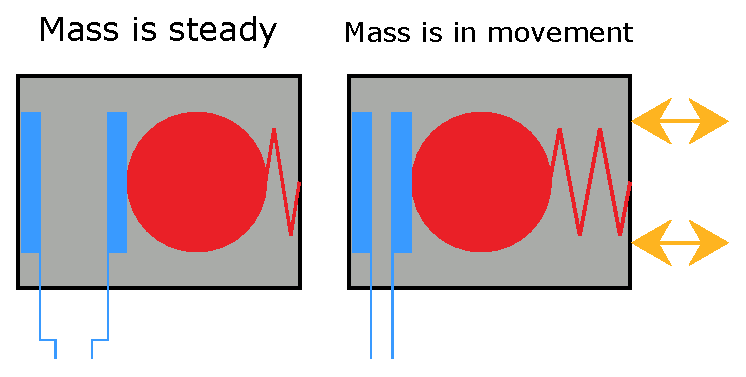
\includegraphics[width=0.45\textwidth]{Chapters/2CHP/Diagrams/capacitiveacc.eps}
    \caption{Illustration of the working principle of capacitive accelerometer}{}    
    \label{fig:wcapacitiveacc}
\end{figure}
In piezoelectric accelerometers, the function principle is similar to the previous, the mass is attached to the piezoelectric and when it moves causes a deformation. The resulting signal from the deformation is the result of the piezoelectric effect. A piezoelectric consist in two metal plates with piezoceramic material between them, usually a quartz crystal. To produce electricity, the piezoceramic material needs to be under stress, that is, to be compressed or squeezed. This caused a voltage different the two metal plates, this is the result of the collection of charges produced in the piezoceramic material.
%%Insert here
\begin{figure}[]
    \centering
    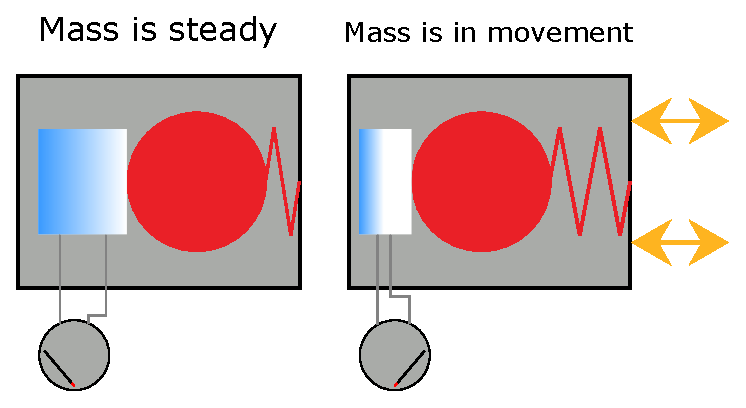
\includegraphics[width=0.45\textwidth]{Chapters/2CHP/Diagrams/piezoresistiveacc.eps}
    \caption{Illustration of the working principle of a piezoresistive accelerometer}{}    
    \label{fig:wpiezoresistiveacc}
\end{figure}
All the type of accelerometers mentioned have one problem, that is the fact that they aren't practical to use in certain application, as an example a small electronic device. For that, is used the so called MEMS (Micro Electro Mechanical Systems) accelerometers, this type of accelerometer is a combination of electrical and mechanical device, mounted on a silicon chip, this is one advantage of this type of accelerometers, the can be very produced in very small sizes, to allows their application in different types of electronic devices. The functioning of this type of accelerometer can be explained quite easily, an electrode is between two other electrodes, there is a air gap between these two and a small insulation to prevent direct contact between the middle electrode and the other two, on the top and the bottom. The middle electrode is connected with a cantilever, rigid enough to hold his position, but flexible enough to allow the move when the accelerometer moves or tilts, the cantilever is connected to outside of the chip, this is used to measure the difference of capacitance between the middle electrode and the electrodes at the top and at the bottom, the capacitance changes every time the middle electrode moves or tilts.
 %%insert the image here as a example, get it from https://www.explainthatstuff.com/accelerometers.html
 \begin{figure}[]
    \centering
    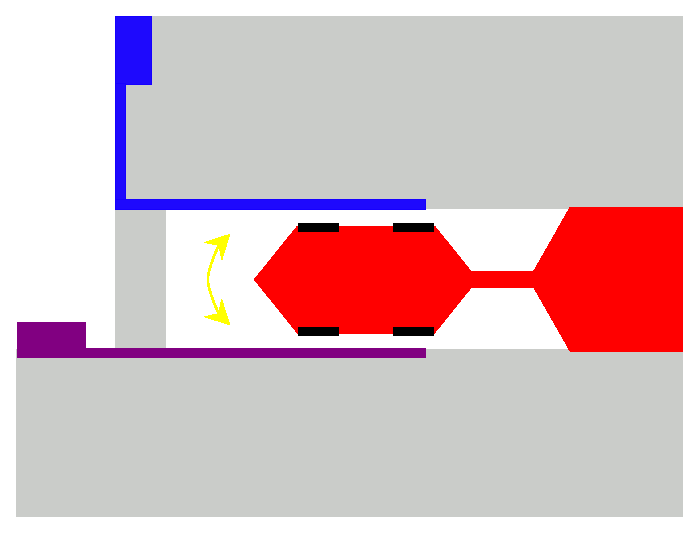
\includegraphics[width=0.45\textwidth]{Chapters/2CHP/Diagrams/memsacc.eps}
    \caption{Illustration of the working principle of a MEMS accelerometer}{}    
    \label{fig:wmemsacc}
\end{figure}
This type of accelerometers brought important advantages, being their low cost and their small size the most important of it. On the other hand, the use of this devices for condition monitoring is restricted to a small bandwidth, restricted to a few kHz, and it cannot be used to in applications that require lower noise over higher frequency ranges \cite{WhatYouNeed,HowAccelerometersWork2009}.

\clearpage
\printbibliography[heading=subbibliography]
\addcontentsline{toc}{section}{References}

%%%%%%%%%%%%%%%%%%%%%%%%%%%%%%%%%%%%%
% AV1 Video Codec
\cleardoublepage
\chapter{System Architecture} \label{chap:sysArch}
\todo[inline,color=red!40]{*Chapter Introduction}
\todo[inline,color=blue!40]{*1-System Elements}
\todo[inline,color=blue!40]{     *1-The sensors/Actuator}
\todo[inline,color=blue!40]{     *2-The processing Unit}
\todo[inline,color=blue!40]{     *3-Processing type?}
\todo[inline,color=blue!40]{*2-Architecture proposal}
\todo[inline,color=blue!40]{*3-Approach to the problem}
\section{System Elements}
In order to develop a system that is able to properly measure and return an good approximation of the liquid level in the LPG bottle, is necessary to identify the elements that must be present in the system. With this information, we must be able to properly chose the components to the system, to develop a solution that fits in the purpose of the work. In Chapter \ref{chap:stArt}, several methods/techniques were presented to measure the liquid level inside a LPG bottle, from those the choice fell to the development of a system that analyses the transversal vibration in the LPG bottle, with this in consideration is easier to define the elements that should be part of the system. 
\subsection*{Actuator}
This element is  responsible for the stimulation of the system, is very important that the chosen actuator is capable to produce the transversal vibration in the system. For this specific case, were presented two different methods for that purpose.
\subsection*{Sensor}
The amount of sensors that can be used to measure the vibration, not specific to this case only, is very wide. There were presented several types of sensors already, but when choosing a specific one it must be taken into consideration aspects like is practical application, in this case, the dimensions of the sensor, his cost and the coupling with the system to be measure, as an example. Other aspects that should be taken in consideration when choosing the sensor, are specific to the sensor itself and may vary from one to another, is not relevant to specify them. 
\subsection*{The Processing Unit}
The selection of the processing unit is quite important, since is the "brain" of the entire system. First of, is responsible for capturing the signal from the sensors, process the signals and at the end being able to return to the user some information, relevant for the application, for this particular application must return some data that is proportional to the liquid level. The processing unit in this case must be equipped with different types of I/O ports, for the specific case, the most important are the ADC for converting the continuous time signal to a discrete signal. Beside the I/O, the system must have the computational power to perform any type of mathematical tasks needed in the signal processing, isn't necessary to have a dedicated DSP hardware, but should be able to perform those tasks in a reasonable period of time.  
%Not sure if it should be here
\todo[inline,color=red!40]{Should be here?}
\subsection*{Processing Type}
As a signal is converted and stored in the processing unity, the signal is decomposed in two variables, they are the dependent variable and the independent variable, the first is usually related with the amplitude of the signal and the other with the sample and overall can be seen as the output of a sensor at a certain moment of time. While this data can be used to return a visual information about the state of the sensor, is not the only way, is often used the frequency domain, to determine patterns in the response of the same sensor, that aren't clear in a time domain visualization.

\section{Architecture proposal}
The system architecture consist in the union of the elements mentioned, to obtain device capable of measure what is intended to. The device itself should be attached in each LPG bottle, to be able to return to the user the liquid level inside. The figure \ref{fig:systemArch} is a illustration of the system elements on the device.\\
\begin{figure}[!htb]
    \centering
    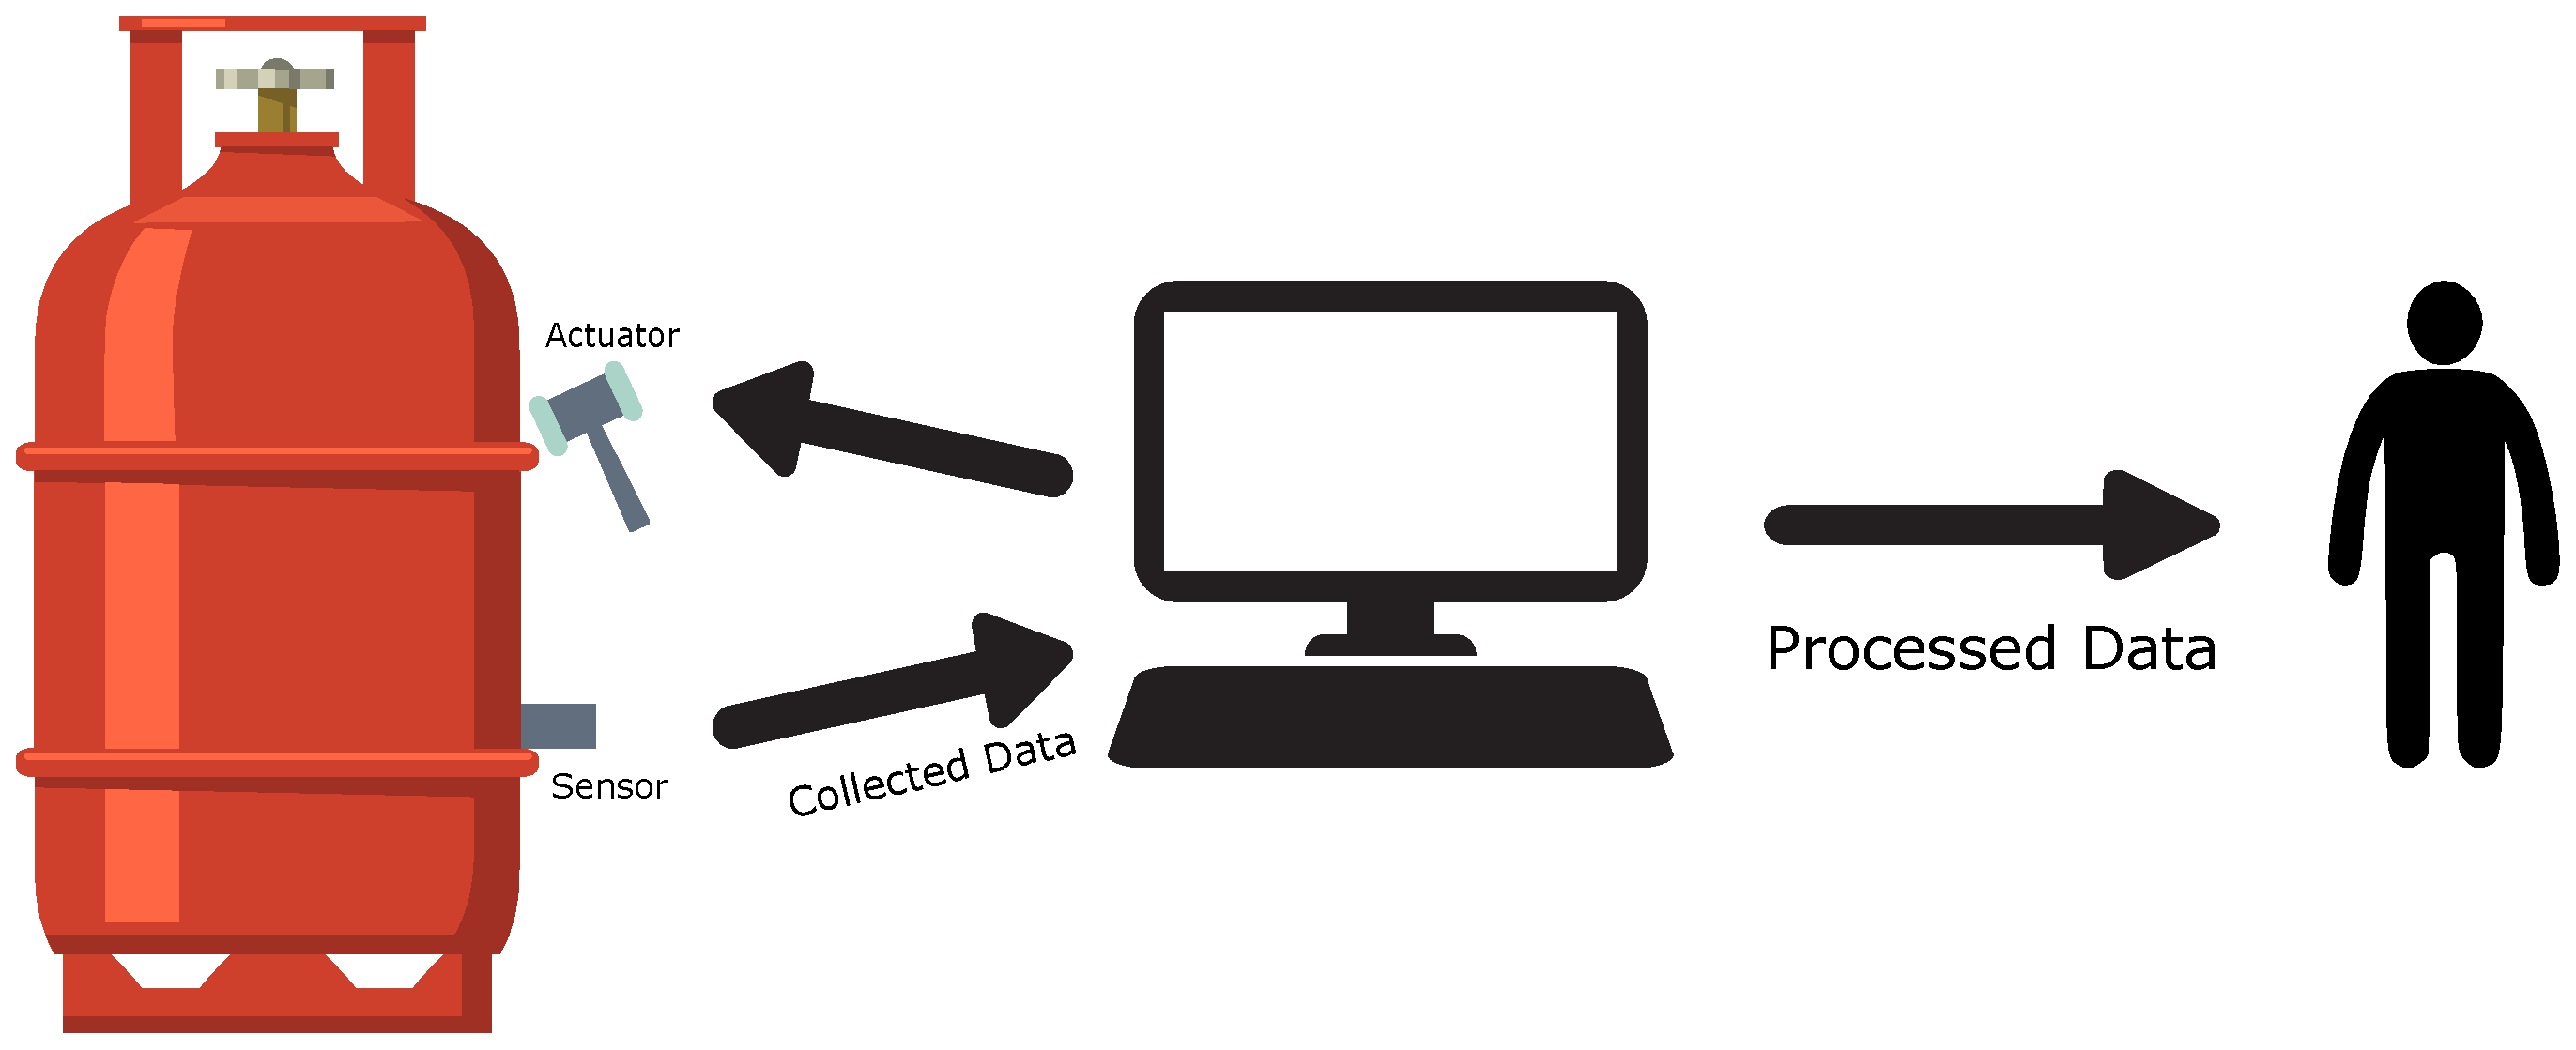
\includegraphics[width=0.55\textwidth]{Chapters/3CHP/Images/bottleBaseAct.eps}
    \caption{Basic architecture of the liquid level measuring device}
    \label{fig:systemArch}
\end{figure}
In the device, the processing unit is responsible for the control of the system as well, the unit is responsible for trigger the actuator in the first place, when this happens the hammer hits the side surface of the LPG bottle and thus the vibration is produce. In the mean time, the process unit starts to convert the signal from the sensor and store that value. Then the recorded data must be processed, in order to return to the user the desire information. Ideally, this procedure would occur once or twice a day, unless a manual measure was requested by the user, but for the purpose of the development of the device, the main purpose is to, in a first stage to get information and being able to associate the same information to the liquid level.\\
The chosen method to process the information, is throw the analysis of the acquired data in the frequency domain, for that a FFT is the chosen method to process the data and later be able to observe and associate the same information with the liquid level. A brief and visual description of the flow of how the process is suppose to occur in the processing unit is illustrated in  
\begin{figure}[!htb]
    \centering
    %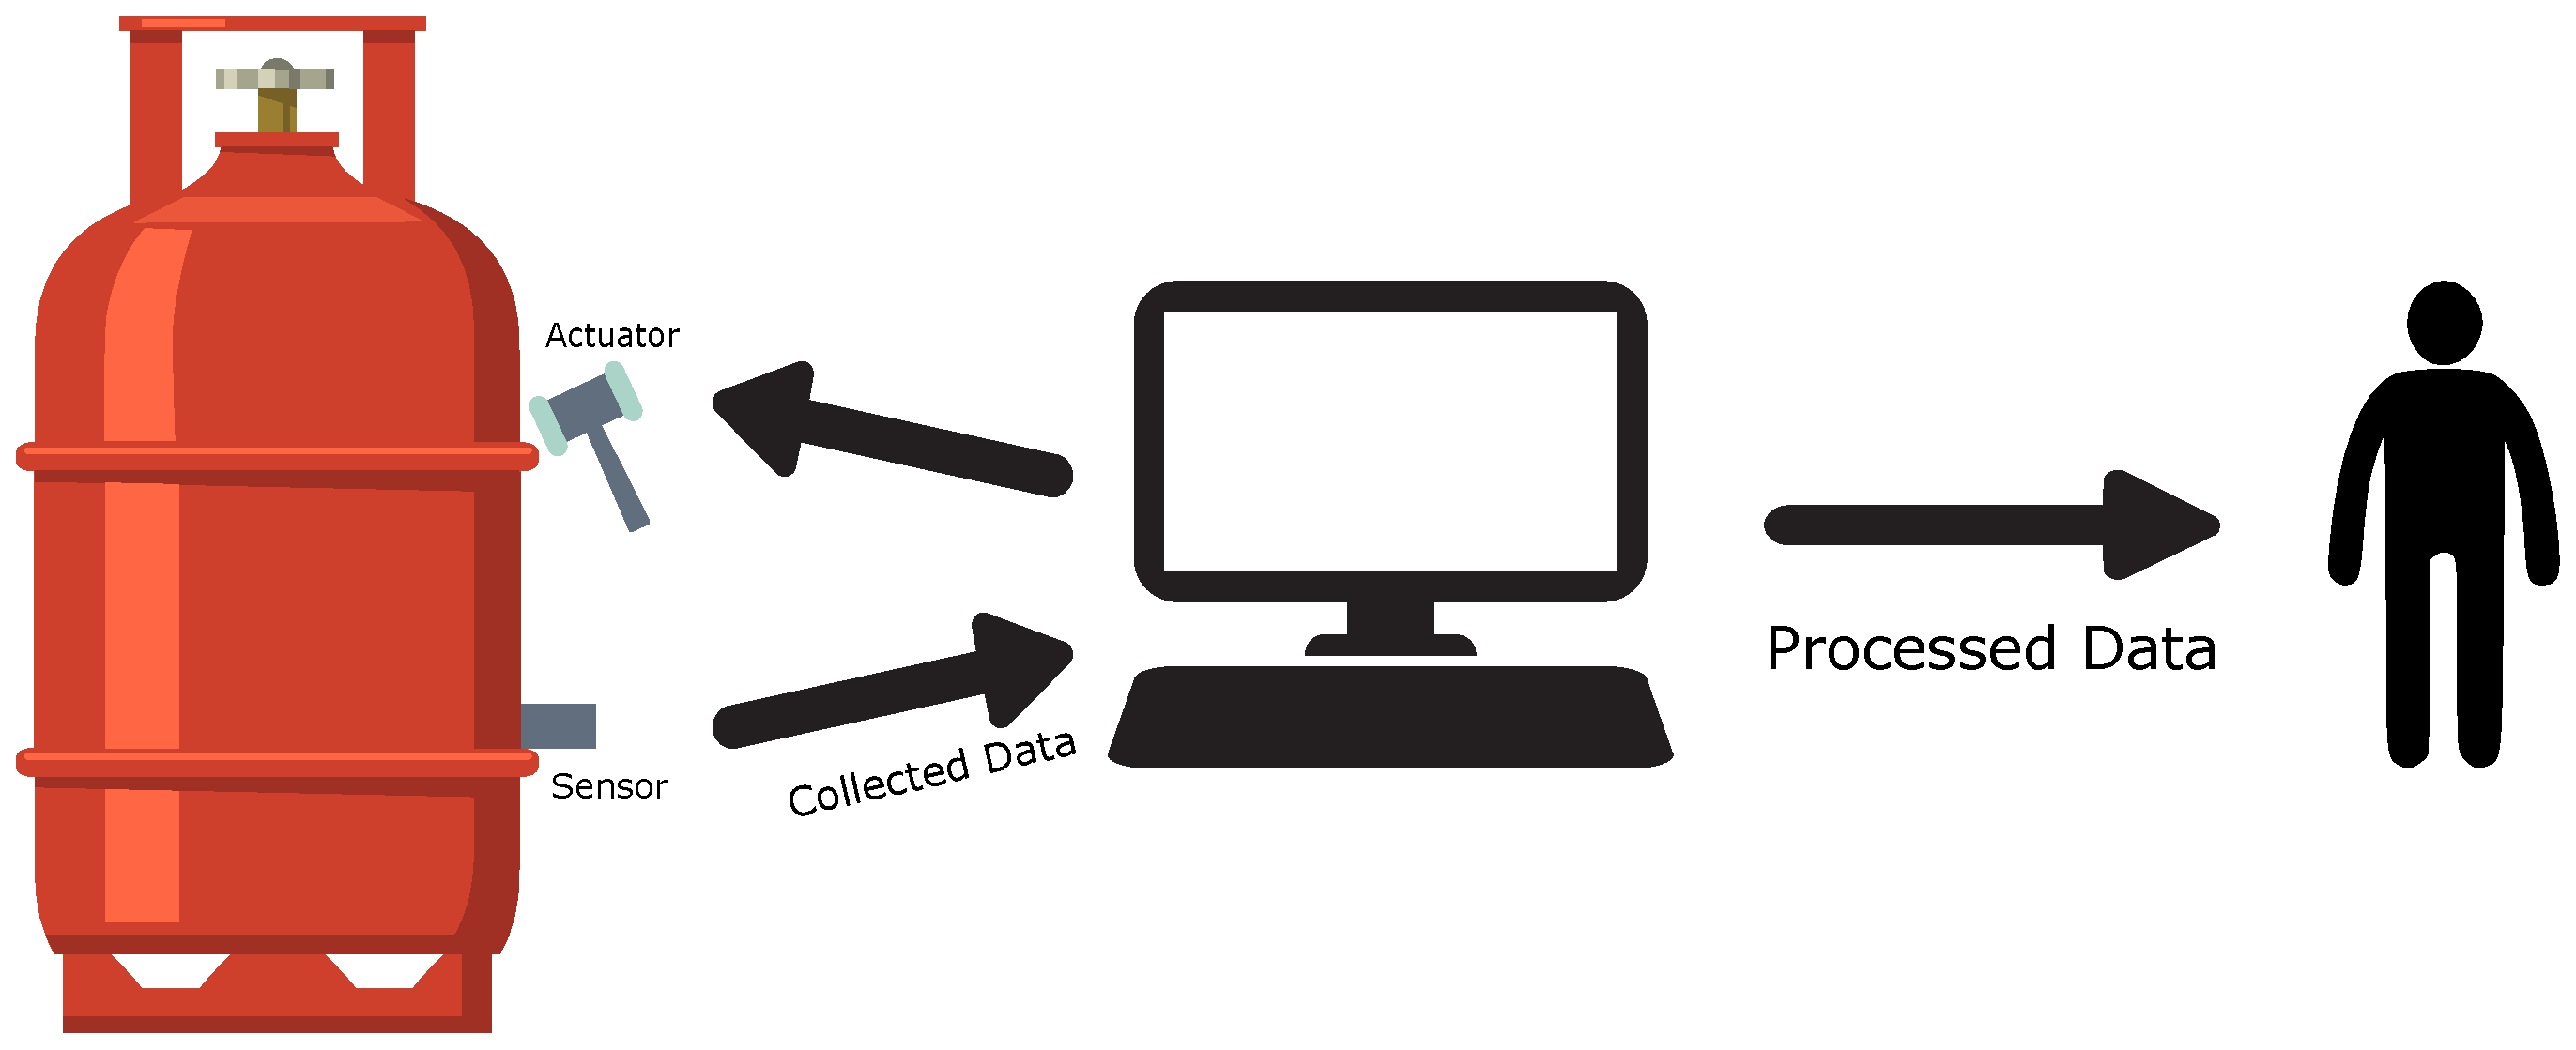
\includegraphics[width=0.65\textwidth]{Chapters/3CHP/Images/bottleBaseAct.eps}
    \caption{Proposed diagram for the device operation}
    \label{fig:systemSWFlow}
\end{figure}\\
\todo[inline,color=red!40]{Should I explain the diagram, or isn't necessary from the explanation before the ilustration?}

\section{Problem Approach}
The approach to obtain a solution and hopefully a device capable of measuring correctly the LPG liquid level will be split in two main phases, each one of them with a different purpose, they are the study of behavior of the system to a external stimulation and the development of the solution for this case. In the two phases the Hardware selection will be different, but on the other hand to what concerns the data processing will be a mixture of different approaches.
In the first stage and in order to understand the behavior, limit the range of analysis of the data and define to the LPG bottle a maximum and minimum value of liquid, it will be used a hammer, a microphone and a computer installed with MatLab, this will allow to capture the sound produced when hitting the side surface of the LPG bottle, and process it in MatLab with the FFT function to analyze the spectrum of the acquired data.
The second stage will be divided in several smaller steps, so is possible to mislead any source of problems. In this stage the microphone will be replaced with two sensors, with the same purpose, in a first stage the hammer will continue to be used as a stimulation method, although later will be replaced with a solenoid, in order to perform automatically the trigger and the signal acquisition. In the same way, in the beginning MatLab will still be used to process the data, but later is to use a microcontroller for that purpose, although for capturing the signals from the sensors, a microcontroller will be used as the interface, and then send the data to the computer. The reason for this is that this way is easier to understand the type of signals acquired from the sensors and how is the proper way to process this data later, on a implementation, avoiding skipping steps.
\todo[inline,color=red!40]{Should  I add a time-table for the approach?}

%everything bellow this will later be migrated to a different chapter - Don't forget to change
\section{Introduction}
%check if the last section of the previous chapter is the more appropriate to use here
%a brief sum of what is going to be presented in this chapter, i.e., first the presentation of the sensors, then the micro controller in use, them the circuits, and at the end the mounting for each case. For what is related to the accelerometer and piezo, both the setups, the simplest and with the pieces.
\section{Hardware selection}%%change this section name later
The analysis through vibration, is the chosen approach to measure the amount of liquid gas inside the LPG bottle, since the stimulation of the system is by hitting in the surface of the bottle, beside the vibration this will produce a characteristic sound as well. From this, 3 different sensors where chosen to acquire the signals when hitting the surface of the LPG bottle, they are a microphone, a piezoelectric sensor and a MEMS accelerometer.\\
In all the cases, when hitting the surface of the bottle with a hammer, this will produce a characteristic vibration and sound, in order to characterize the response of the system to the hit of the hammer, the first analysis is made with a microphone, after this the sensors will be chosen and the design the appropriate circuit to capture the same signal.
%%Incomplete, must be able to include references to the microcontroller and the circuits

\subsection{Microphone}
Before trace a curve is important to understand which one is the best point to acquire data, when hitting the surface of the bottle. For that, different point in the bottle were chosen to determine the point. After this several measurements must be conducted in order to have a reliable source of information and trace a curve for the system response.\\
The point considered are in the side surface of the LPG bottle as illustrated in the following image:
%%insert here a description of the points considered
To make those measurements a setup must mounted with a microphone, to capture the sound produced and process it. The setup is quite simple, consisting in a microphone and a computer installed with MatLab. The microphone in use is from a phone and to connect it with the computer an software called \textit{WO Mic}, this allows to used the microphone of the phone in real-time. The software must be installed in both devices, in the phone the software is available for Android and IOS, is responsible to transmit what is captured from the microphone. In the computer the client application and a virtual device must be installed to use the Phone in the computer to perform any type of tasks, this connection can be made by USB, Bluetooth, Wi-Fi and Wi-Fi Direct.\\ 
In order to save what is captured from the microphone, the software is split in three main block with different purposes, the \textit{WO Mic App} runs in the Phone, samples the input of the microphone and transmit it to the computer, the \textit{WO Mic Client}, runs in the computer, connect to the app in the phone, and receive the data from the microphone, which is transmitted to the \textit{WO Mic Virtual Device} on which a real microphone device is simulated and provides the audio to any application or program in the computer\cite{WOMicFREE}:\\
\begin{figure}[!htb]
    \centering
    \includegraphics[width=0.65\textwidth]{Chapters/3CHP/Images/WOMICDiag.png}
    \caption{Flow of data in the components of the software\cite{WOMicFREE}}
    \label{fig:diagramWOMIC}
\end{figure}
In addition to this, is also necessary to install the drivers of the phone in use, if the connection is made over USB.\\
To save the acquired data, MatLab was used to record the data of the microphone from the desire time and saved in ".txt" files for further analysis. 
%%The following two paragraphs must go in other section
%%Insert flux gram here for a easy explanation and perception of the flow of information
A script in MatLab was developed in order to perform this measurements and the capture is made once at a time, but not all configurations are done over this script. To start, the phone is connected over USB to the computer, in the application at phone the transport selected must be \textbf{USB}, on the app settings and after that started the application, in the top right play shape button. 
%%Insert here instructions
In the computer the client software must be initialized and connected to the phone in the following order \textit{\>Connection\>Connect...} a new window will open, on which the \textbf{USB} must be selected as transport type and finalizing by pressing \textit{Connect}. In MATLAB the input correspondent to the microphone must be selected.\\
When this is done, the script runs and starts to record data from the microphone, for the desire amount of time. When the microphone starts to record, the surface of the LPG bottle is knocked and the captured signal is saved.
%%
%%
\subsection{Coupling} 

% \begin{figure}[!htb]
%     \centering 
%         \begin{subfigure}[c]{\textwidth}
%             \centering
%             \input{Sections/3Transforms/Images/DFTSymmetry.tex}
%             \caption{}
%             \label{subfig:dft}
%         \end{subfigure}
%         \begin{subfigure}[c]{0.45\textwidth}
%             \centering
%             \input{Sections/3Transforms/Images/DCT1Symmetry.tex}
%             \caption{}
%             \label{subfig:dct1}
%         \end{subfigure}
%         \begin{subfigure}[c]{0.45\textwidth}
%             \centering
%             \input{Sections/3Transforms/Images/DCT2Symmetry.tex}
%             \caption{}
%             \label{subfig:dct2}
%         \end{subfigure}
%         \begin{subfigure}[c]{0.45\textwidth}
%             \centering
%             \input{Sections/3Transforms/Images/DCT3Symmetry.tex}
%             \caption{}
%             \label{subfig:dct3}
%         \end{subfigure}
%         \begin{subfigure}[c]{0.45\textwidth}
%             \centering
%             \input{Sections/3Transforms/Images/DCT4Symmetry.tex}
%             \caption{}
%             \label{subfig:dct4}
%         \end{subfigure}
%         \caption{Sequences generated in the first step of Table \ref{tab:DFTDCT}for the DFT and different DCTs. Filled dots correspond to the original sequence ((a) - \emph{DFT}; (b)) - \emph{DCT-I}; (c)) - \emph{DCT-II}; (d)) - \emph{DCT-III}; (e)) - \emph{DCT-IV}).}
%     \label{fig:2NSeq}
% \end{figure}
% \begin{lstlisting}
%     ./aomenc <INPUT-FILE> -h <HEIGHT> -w <WIDTH> -o <OUTPUT-FILE> --limit=10 -p 1 --cpu-used=8 --i420 --q-hist=64 --end-usage=q --cq-level=<CQ-LEVEL>
% \end{lstlisting}
\clearpage
%\printbibliography[heading=subbibliography]
%\addcontentsline{toc}{section}{References}

%%%%%%%%%%%%%%%%%%%%%%%%%%%%%%%%%%%%%
% Developed Architecture
\cleardoublepage
\chapter{Hardware}\label{chap:hardware}
% To do: 
% Color Scheme
% Red - Not started
% Yellow - In progress
% Blue - Done, under approval
% Green - Done and approved
\todo[inline,color=red!40]{*Latter add Section for the actuator}
\todo[inline,color=red!40]{*Chapter Introduction}

\todo[inline,color=yellow!40]{*1 - Selection}
\todo[inline,color=blue!40]{ a) Microphone}
\todo[inline,color=blue!40]{ b) Accelerometer}
\todo[inline,color=blue!40]{ c) Piezoelectric}
\todo[inline,color=blue!40]{ d) Microcontroller}
\todo[inline,color=blue!40]{ e) Solenoid}

\todo[inline,color=yellow!40]{*2 - Design} % Missing review
\todo[inline,color=red!40]{ a) Accelerometer}
\todo[inline,color=blue!40]{ b) Piezoelectric}
\todo[inline,color=blue!40]{ c) Solenoid}

\todo[inline,color=blue!40]{*3 - Capture/Coupling}
\todo[inline,color=blue!40]{ a) Microphone}
\todo[inline,color=blue!40]{ b) Accelerometer} % missing illustration with the magnet glued to the accelerometer
\todo[inline,color=blue!40]{ c) Piezoelectric}
%% Writing %%%%%%%%%%%%%%%%%%%%%%%%%%%%%%%%%%%%%%%%%%%%%%%%%%%%%%%%%%%%
 
\section{Selection}
\subsection{Microphone}
With the interest of understanding what is the system response to an external stimulation, it is needed a simple method to record that response. The easiest way to do that is by using a microphone to capture the sound produced when hitting the side surface of the \acrshort{lpg} bottle. By the time this study started, the material needed wasn't available, for this case a microphone and a soundboard, an alternative was necessary.

Although there are various alternatives for it, like the embedded computer microphone, or an external microphone, none of those were able to properly capture the sound and be mounted in a practical setup. The alternative for this solution was recurring to the use of the microphone of a regular phone.  The phone itself is connected via USB to the computer, on which additional software was installed to allow access in real time the microphone of the phone.  In figure 4.1 is an illustration of the connection between the microphone of the phone and the computer.
\begin{figure}[]
    \centering
    %\includegraphics[width=0.65\textwidth]{Chapters/3CHP/Images/WOMICDiag.png}
    \caption{Physical connection of the phone microphone to the computer}
    \label{fig:MicConnectio}
\end{figure}
\subsection{Accelerometer}
As already mentioned in section \ref{sec:VibSens}, there are various types of accelerometers, however the choice of the one to use depends on various factors, for this particular application is important that the accelerometer in use has a low cost and a small size, for the future application. With this in mind the choice declines over MEMS accelerometers, that are smaller when compared with piezoelectric accelerometers.

The type of \acrshort{mems} accelerometers available is very wide, some of them started to be used in applications that usually uses piezoelectric accelerometers, like \acrshort{cbm}, \acrshort{shm}, \acrshort{ahm}, \acrshort{vsm} and \acrshort{iot}. When selecting the accelerometer it is important to take into consideration some parameters, which are responsible to determine the category of the accelerometer, they are the application, the bandwidth and the range. Although there is no standard for the category on each accelerometer fits in, Analog Devices has one document where they divide their products in different categories, with the type of application used in each one of them, featuring a description of the key parameters, that must be taken into consideration when selecting the appropriate accelerometer.
\begin{figure}[]
    \centering
    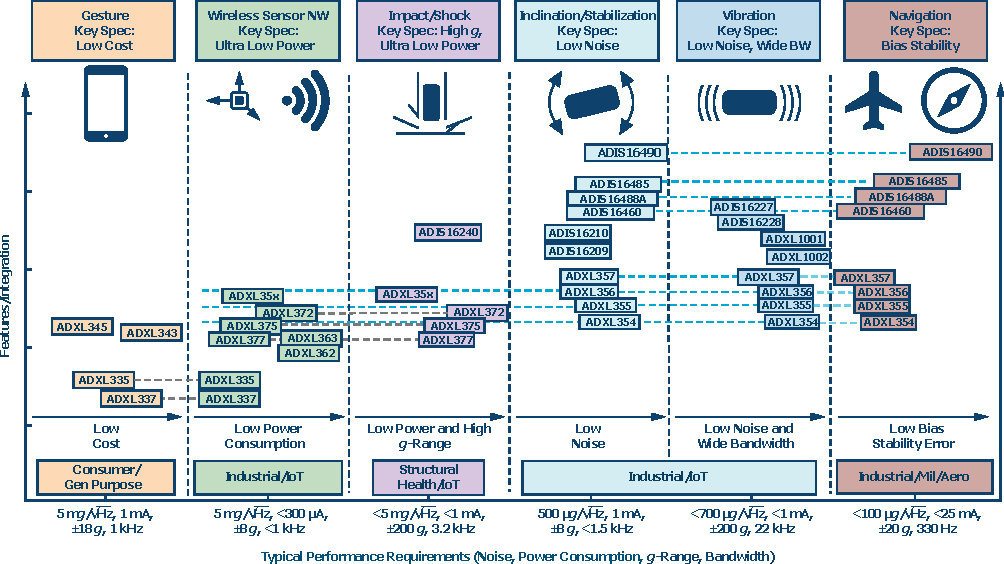
\includegraphics[width=1\textwidth]{Chapters/4CHP/Figures/adTable.pdf}
    \caption{Application landscape for a selection of Analog Devices MEMS accelerometers}
    \label{fig:adtable}
\end{figure}
The \acrshort{mems} accelerometers, from Analog Devices, are divided in two families, the ADXLxxxx and the ADIS16xxxx. The last offers different advantages when compared with he first, more like a plug-and-play solution with features like factory compensation, embedded compensation and signal processing. This family obviously has one of the features that has particular interest for the application, in this case the fact that has signal processing on the accelerometer, on the other hand this comes with a price, and this family of products has a higher cost. So is necessary to define the key specifications of the accelerometer, in order to properly chose one\cite{AnalogDialogue51102017}\cite{AnalogDialogue51112017}.

The final purpose is to have a cheap and portable prototype, that is capable of accurately measuring the vibrations and determine the liquid level, this implies that his bandwidth covers the spectrum of frequency on which the curve of the relation liquid level vs frequency is. With this the key specifications are the low cost, low power and his bandwidth must close to 2kHz, determine as maximum frequency for a mechanical vibrations in \ref{tab:sampRat} and latter proved in the results obtained by \citeauthor{wuLiquidLevelDetector2014b} as described in \ref{sec:LPGModel}. Considering these specification, some models where chosen, that integrate this criteria, as follows:
\begin{table}
    \centering
    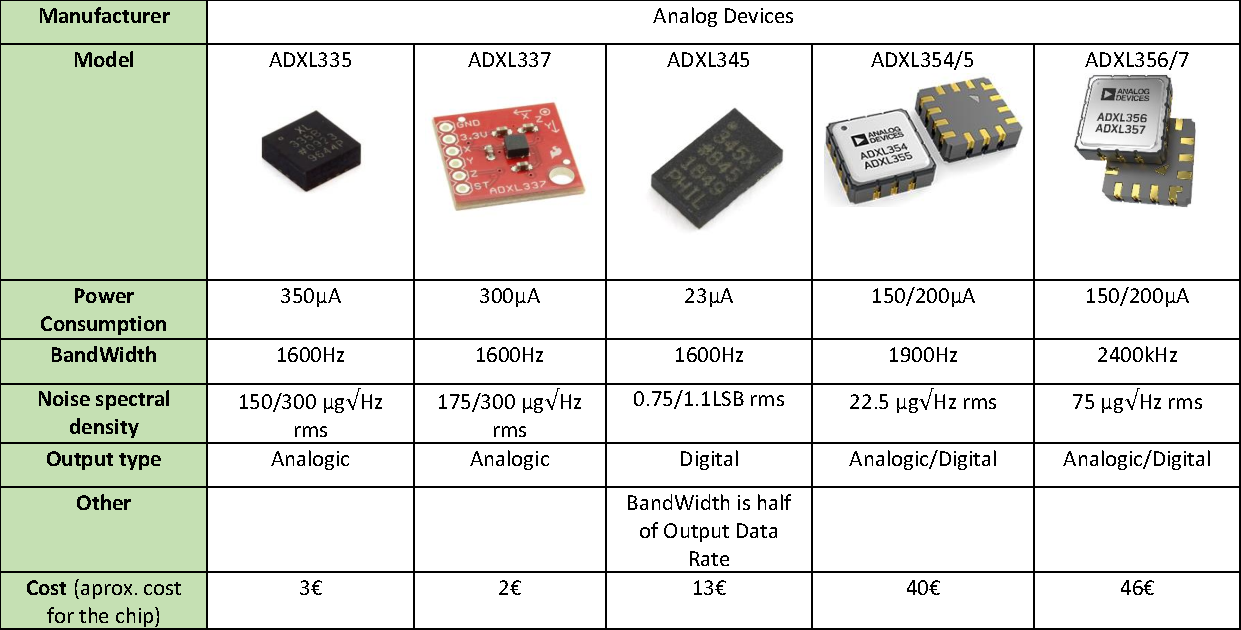
\includegraphics[width=1\textwidth]{Chapters/4CHP/Figures/accTable.pdf}
    \caption{Key specifications of MEMS accelerometers}
    \label{tab:acctable}
\end{table}
Although it doesn't accommodate entirely the specifications but since it was already available for use, the choice fell to the ADXL335. This model offers a low power consumption, of around 350$\mu$A, his bandwidth is adjustable with a single capacitor per axis, from 0.5 to 1600 Hz for X and Y axis and 0.5 to 550Hz for Z axis. Beside this the accelerometer itself is very cheap, with a price starting at 3€. To properly acquire the data from this sensor and process it, is necessary to integrate it with an amplifier circuit and a microcontroller, on which more details will be explained further ahead.
\subsection{Piezoelectric}
%%Missing the images and the review
There are several types of piezoelectric constituents, a defining factor of the type of material used in the piezoelectric, is his application. The most commonly used in vibration measurement is \acrshort{pvdf} as polymer and \acrshort{pzt} as ceramic. The reason for that is due the fact that they can measure either high or low frequencies. This sensor usually produces charges according to the applied pressure, the tension generated at the output is related with the amount of charges generated. In a electric point a view this is a sensor with a high-impedance, therefore is necessary a amplifier circuit with a high input impedance and with a high \acrshort{snr} relation. For piezoelectric it is usual to use a charge amplifier, that already fills these requirements.

In the developed work, was used two different \acrshort{pzt} piezoelectric, with different dimensions, one with a diameter of 27mm and the other with a diameter of 12mm.

\begin{figure}[]
    \centering
    \begin{subfigure}{0.45\textwidth}
        \centering
        \includegraphics[width=\linewidth]{Chapters/4CHP/Figures/piezo27mm.png}
        \caption{}{}
        \label{subfig:piezo1}
    \end{subfigure}
    \begin{subfigure}{0.45\textwidth}
        \centering
        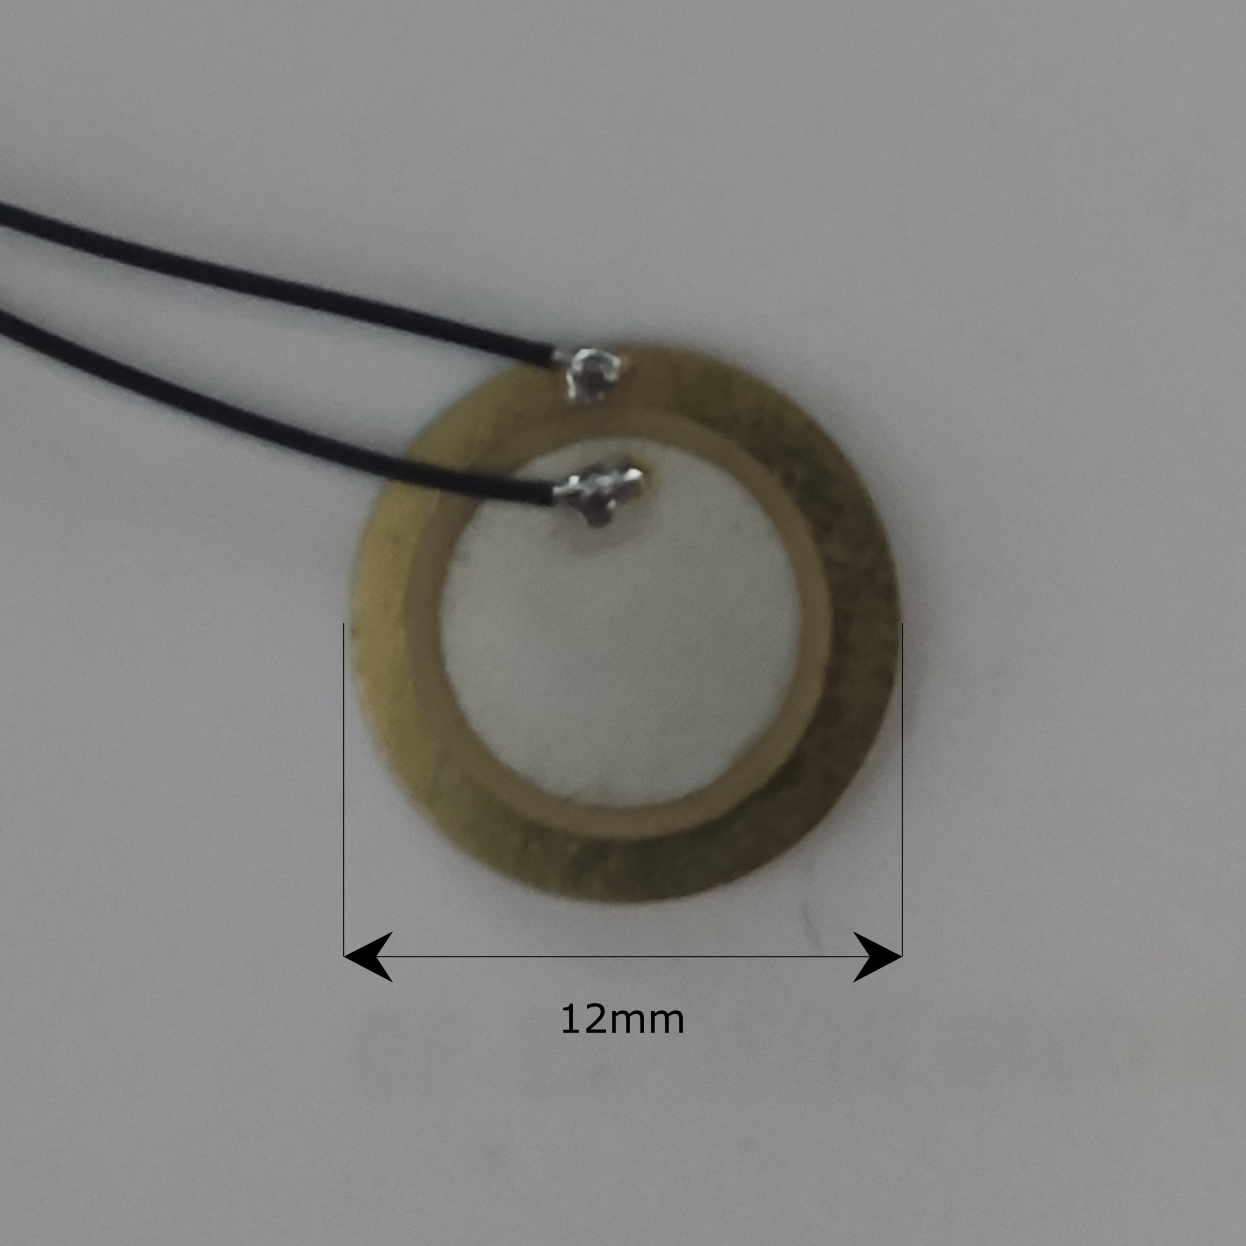
\includegraphics[width=\linewidth]{Chapters/4CHP/Figures/piezo12mm.png}
        \caption{}{}
        \label{subfig:piezo2}
    \end{subfigure}
    \caption{Piezoelectric sensors used}{}
    \label{fig:UsedPiezos}
\end{figure}
The use of a piezoelectric, is not only a cheaper option, when compared with the accelerometer, but also allows to pursue a different approach. This is related with the stimulation technique of the system, that can replace the hitting to a different technique that uses the piezoelectric, although this option won't be considered during the development of the work. 

\subsection{Microcontroller}
When selecting the microcontroller, it is important to have some specifications in mind, as in the perspective of a future implementation, one that is quite important is the performance, the cost, as well as the power consumption. There is a large variety of products that most certainly would fit in these specifications. The selection of this it took in consideration those characteristics and fell to one from \acrlong{ti}, the model of the chosen microcontroller is the MSP-EXP430FR2433, his characteristics are the following:
\begin{itemize}
    \item 16-bit \acrshort{risc} processor with a clock frequency up to 16MHz;
    \item 15KB of program and 512B information \acrshort{fram}, 4KB \acrshort{ram};
    \item 8-channel 10-bit \acrshort{adc};
    \item Four 16-bit Timers, 16-bit counter-only \acrshort{rtc};
    \item 32-bit Hardware-Multiplier;
    \item Two \acrshort{eusci}\_A, supports \acrshort{uart}, \acrshort{irda} and \acrshort{spi} and one \acrshort{eusci}\_B, supports \acrshort{spi} and \acrshort{i2c};
\end{itemize}
Beside these characteristics the microcontroller offers different low-power modes, that consume from hundreds of microAmps to a couple of hundreds of microAmps, depending on the mode of operation of the microcontroller. Another thing in consideration, when selecting, is the fact that it is possible to run with a super cap. The performance in this case is not as important as it seams, is not mandatory that operation that would need to be performed must return the result to the user instantly, that means that the results not being in real time won't make much of a difference, anyway if that was the case. There is also a 32-bit Hardware-Multiplier embedded that reduces the use of \acrshort{cpu} time to perform multiplications that would be required\cite{MSP430FR2433DataSheet}. Associated with these characteristics, the price of this microcontroller is very appealing, starting under 2€.

\subsection{Solenoid}
For more constant measurement it is important that when the hitting process is constant as well, for that one a manual hammer is substituted by a solenoid, that when powered for a short period can simulate an impulse in the system, as it happens with the hammer. With that purpose was chosen the SOL01002, the reason is, first this solenoid work with tensions starting at 5V and the other reason is due the fact that is a Push type, which means that when powered the shaft will move and produce the impulse desire.
\begin{figure}[]
    \centering
    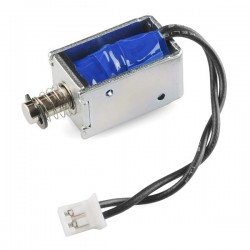
\includegraphics[width=0.45\textwidth]{Chapters/4CHP/Figures/solenoide.jpg}
    \caption{Solenoid used to stimulate the bottle}
    \label{fig:solenoid}
\end{figure}
The downside of using this model, can be the low impact force, it may not be able to produce a strong enough hit that can be detected by the sensors. This factor is just a assumption, along the test, is going to be verify if it happens or not.
\section{Design}
\subsection{Accelerometer}

\subsection{Piezoelectric}
As mentioned, piezoelectric sensors can be used in many fields, for sensing acceleration, vibration, shock or pressure. To what is related to acceleration or vibration, the piezoelectric will output a charge that is a function of his deformation/deflection. For the application in specific, the vibration produce, although is noticeable directly at the piezoelectric output, has a small amplitude which means that needs to be amplified to allow a distinct difference between what is actually the vibration and the output of the piezoelectric itself, is important to properly design a signal conditioning amplifier circuit. \acrlong{ti} has a very clear document explaining how to design charge amplifiers for piezoelectric sensors \cite{bartolomeSignalConditioningPiezoelectric2010}, on which they explain different types of circuits for this application in specific, with the advantages and disadvantages. The simplest model of this type of circuit is as follows: 
\begin{figure}[]
    \centering
    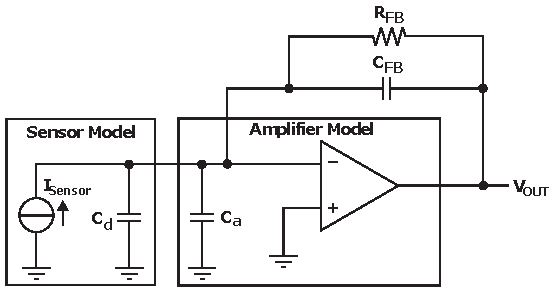
\includegraphics[width=0.45\textwidth]{Chapters/4CHP/Figures/singleenddedchargeamp.pdf}
    \caption{Charge Amplifier for signal conditioning}
    \label{fig:ChargeAmpSimp}
\end{figure}
Two important things to consider is the bandwidth and the gain of the circuit. In the first case, the circuit functions as a High-Pass Filter which means that when selecting the feedback resistor and capacitance, their values must be selected to keep a low pole in the filter.
\begin{equation}\label{eq:fhpf}
    f_{HPF} = \frac{1}{2\pi R_{FB}C_{FB}}
\end{equation}
Usually the value of the resistor in use is on the order of hundred of megaohms and the capacitance should be low, the reason is due to the fact that in these circuits the gain is defined by the value of the capacitance, the lower is value, the higher the gain.
\begin{equation}
    Gain = \frac{1}{C_{FB}} (mV/C)
\end{equation}
Another factor that must be taken in consideration is the \acrshort{snr}, this value needs to be maximized. For this circuit in specific, one way to archive this is by increasing the value of $R_{FB}$ as much as possible. To outline this and improve the \acrshort{snr} value is through the use of a differential charge amplifier.
\begin{figure}[]
    \centering
    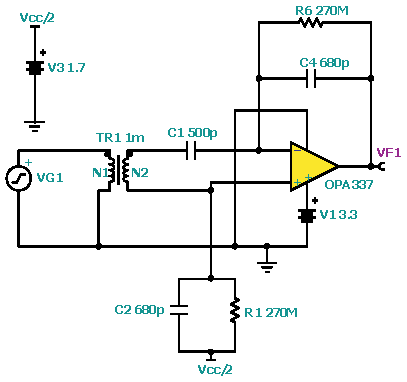
\includegraphics[width=0.45\textwidth]{Chapters/4CHP/Figures/differentialchargeamp.pdf}
    \caption{Differential Charge Amplifier for signal conditioning}
    \label{fig:ChargeAmpDif}
\end{figure}
This circuit offers two main advantages when compared with a simple charge amplifier, the first is related with the gain, in this case has twice the gain of a single-ended input circuit, (while the noise increases only as a square-root function???). The second is due to the fact that these circuits are very sensitive, in a single-ended input one of the terminals injects current while the other is connected to the ground, this will amplify the interference. In a differential input the common-mode signals will cancel each other.

For the practical application, the  circuit in use will be as shown in figure \ref{fig:ChargeAmpDif}, considering the simulation that the document \cite{bartolomeSignalConditioningPiezoelectric2010} presents, mainly those related with the \acrshort{snr}, this seemed to be the suitable choice for the application, since noise is a key aspect when measuring the signal, this is one way of reducing the effect of it. The difference in the circuit in use will be the components, the \acrshort{opamp} in use will be the MCP602 from MicroChip, as for the remaining components, if is consider the information from the document, it can be select the values of 1nF for the capacitors and 100M$\Omega$ for the resistors. With these values the pole of the High-Pass Filter will be set at 1,59Hz and the gain of the circuit 2G(mV/C).
\begin{figure}[]
    \centering
    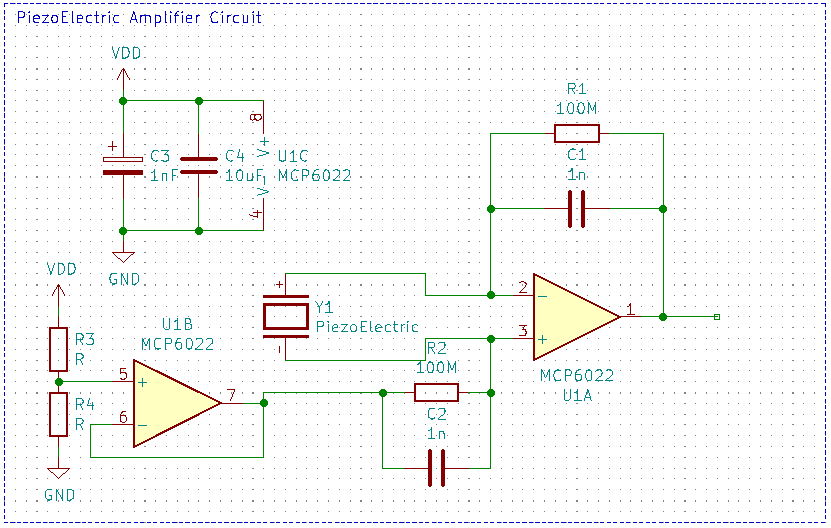
\includegraphics[width=0.45\textwidth]{Chapters/4CHP/Figures/piezoAmpcirc.PNG}
    \caption{Differential Charge Amplifier Schematic}
    \label{fig:ChargeAmpDifSCH}
\end{figure}
Note that,once again, beside being connected in differential mode, the circuit has on its positive input, a fixed input voltage of half the supply voltage of the OpAmp.
\subsection{Solenoid}
The circuit needed for driving a solenoid is very simple, it consists simply in a \acrshort{mosfet}, a diode and a resistor as components. Is needed to pay attention to the used \acrshort{mosfet}, if the solenoid is active by a microcontroller, that is a high output has 3.3V in the specified pin, is needed to be one with a low threshold voltage from the gate to the source. The use of the diode in parallel with the solenoid is to forward the current when the \acrshort{mosfet} is switched off. In figure \ref{fig:solenoidshc} is the schematic of the circuit used to drive the solenoid.
\begin{figure}[]
    \centering
    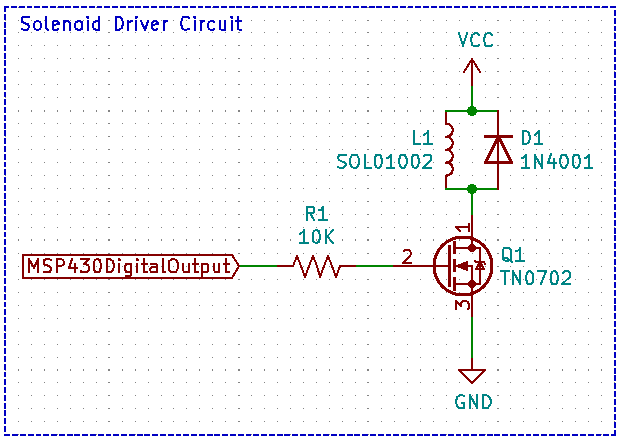
\includegraphics[width=0.65\textwidth]{Chapters/4CHP/Figures/SolenoidDriver.PNG}
    \caption{Circuit for driving the solenoid}
    \label{fig:solenoidshc}
\end{figure}
\section{Capture/Coupling}
\subsection{Microphone}
To position the microphone and acquire the sound produced when hitting the tank surface, the microphone was placed perpendicular to the surface of the tank and as close as possible from it, is also recommended to place it near the hitting point. With caution not to hit the microphone while measuring. The figure \ref{fig:micmount} is an illustration of how the microphone is placed relative to the \acrshort{lpg} bottle.
\begin{figure}[]
    \centering
    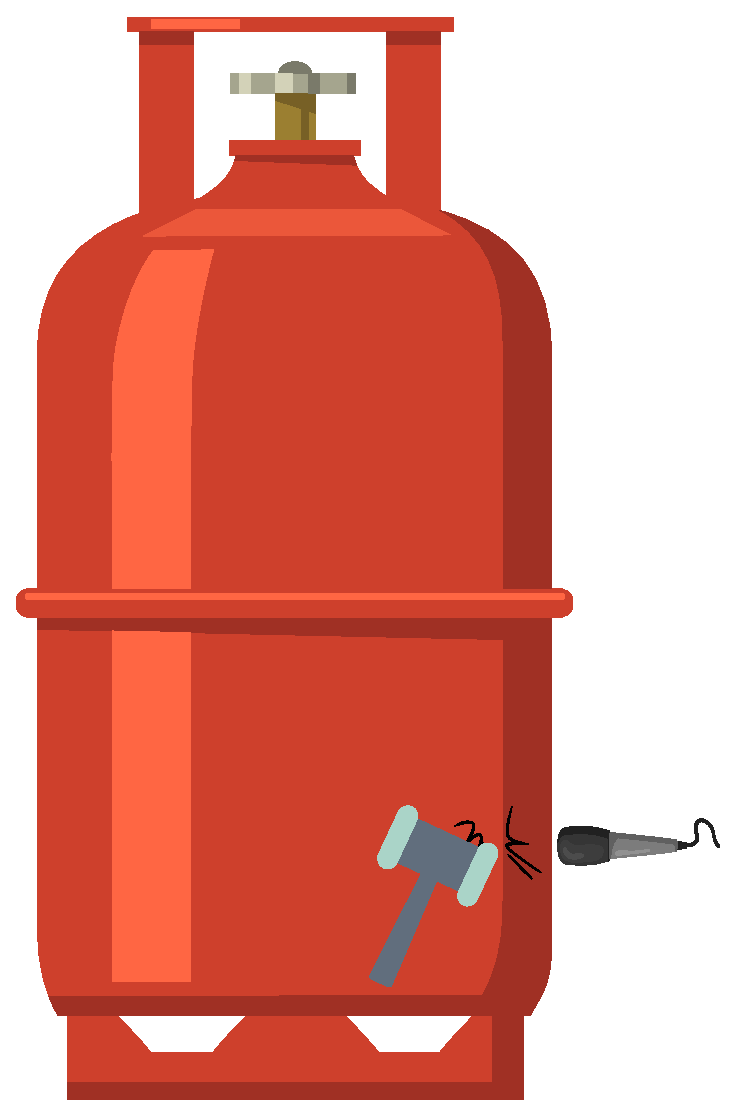
\includegraphics[width=0.3\textwidth]{Chapters/4CHP/Figures/micWimpactHamm.eps}
    \caption{Illustration of the accelerometer mount with a load strap}
    \label{fig:micmount}
\end{figure}
In the practical setup, since it uses the microphone from the phone, the side of the phone where the microphone is, should be faced to the \acrshort{lpg} bottle, usually the bottom part.
\subsection{Accelerometer}
When using an accelerometer for sensing vibration, there are different methods to mount it to the desire surface. Usually in the industry the accelerometer is mounted to the surface with a screw, allowing good contact with the surface, but in the application pretended is not possible to use that method, since that would imply the change in the structure of the tank and the accelerometer in use is not ready for a screw mount. There are other methods to attach the accelerometer to the tank and even though that the examples from \cite{GuidelinesMountingTest} are to accelerometers with a screw mount, their examples can easily adapted to the type of accelerometer in use without any changes in the structure.

The type of mount is quite important in the frequency response of the accelerometer, as well as the surface on which the accelerometer is going to be mounted at. The best results are usually obtained with a stud or screw mount, but that isn't possible since it would require structural changes to the tank, two other options are presented. One of the options is by using an adhesive, this is a possibility, but in a practical mount the surface and the sensor would require different mounting bases, to avoid damaging the sensor and allow to the sensor to be removed any time that is required. Although this is practical to mount, would also require that each tank had already the adhesive for the mount. When compared with the other two mounting methods, this offers worse accuracy in frequency response. The second option is a magnetic mount, although it has a lower frequency accuracy, when the first two methods, stud and screw, this method offers a convenient mount if the structure of the tank is metallic, for this case is advised that the magnet is in a separate piece, to avoid damaging the accelerometer. Magnets with a high pull strengths are better in providing a good frequency response, a system with dual-rail mount is god when the surface that the sensor is mounted on, is curve, but this decreases the operational frequency range of the accelerometer.

For the mount of the accelerometer in the \acrshort{lpg} bottle, will be used a magnet mount, is the most practical mount for a future application. Although in a laboratory environment and for test effects it won't be the only type of mount used. The first mount method will be with a load strap, this will hold firmly the sensor against the wall of the tank, as will be used for the first tests. In figure \ref{fig:mounLoadStrap} is an illustration of the sensor mount.
\begin{figure}[]
    \centering
    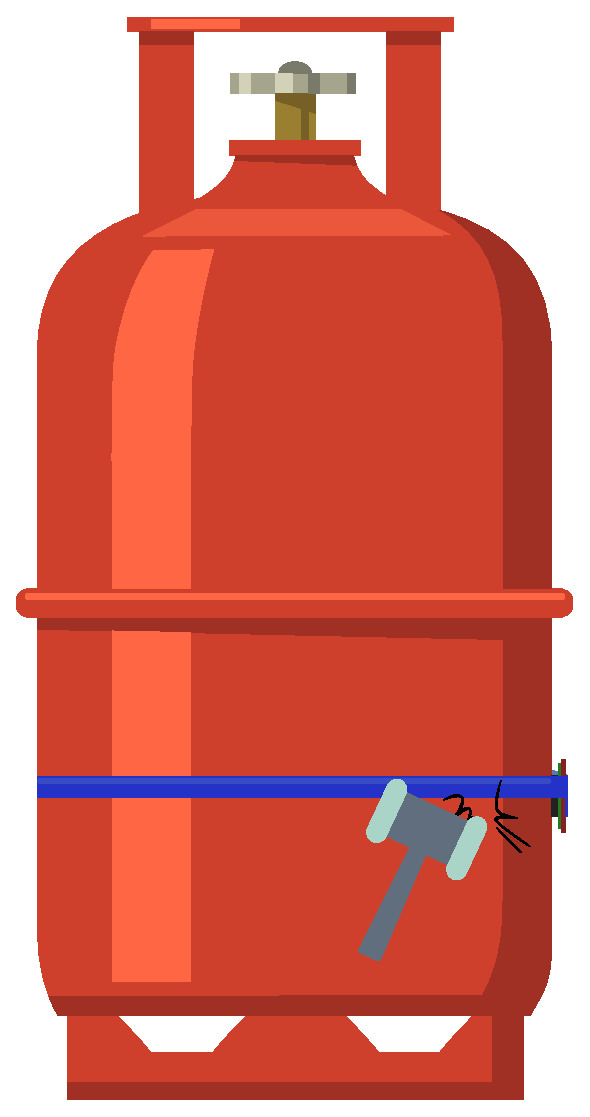
\includegraphics[width=0.3\textwidth]{Chapters/4CHP/Figures/AccLoadStrap.eps}
    \caption{Illustration of the accelerometer mount with a load strap}
    \label{fig:mounLoadStrap}
\end{figure}
For the magnet mount, there are actually two proposals, if by any reason one doesn't produce any results. In figure \ref{fig:mounMagnet} [a] is the ideal option, since it is less invasive for the accelerometer, for the reason mentioned above. In this case, a piece is design to be able to mount with two neodymium magnets at the top and bottom of the piece, this will pull the piece against the wall of the tank, between the two magnets is the necessary space for held the accelerometer, a sponge will be glued to the piece on one side and the other will be glued to the accelerometer, this will be slightly thicker than the piece, that way when the magnets attached the piece against the tank wall, the sponge will be compressed and and the surface of the accelerometer, is expected to be firmly held against the tank wall as well. In figure \ref{fig:mounMagnet} [b], the mount is not ideal, since the neodymium magnet will be glued to the accelerometer surface for a god contact, this may result in best results when compared with the first option, but can damage the accelerometer, when attaching or removing the accelerometer from the tank wall.
\begin{figure}[]
    \centering
    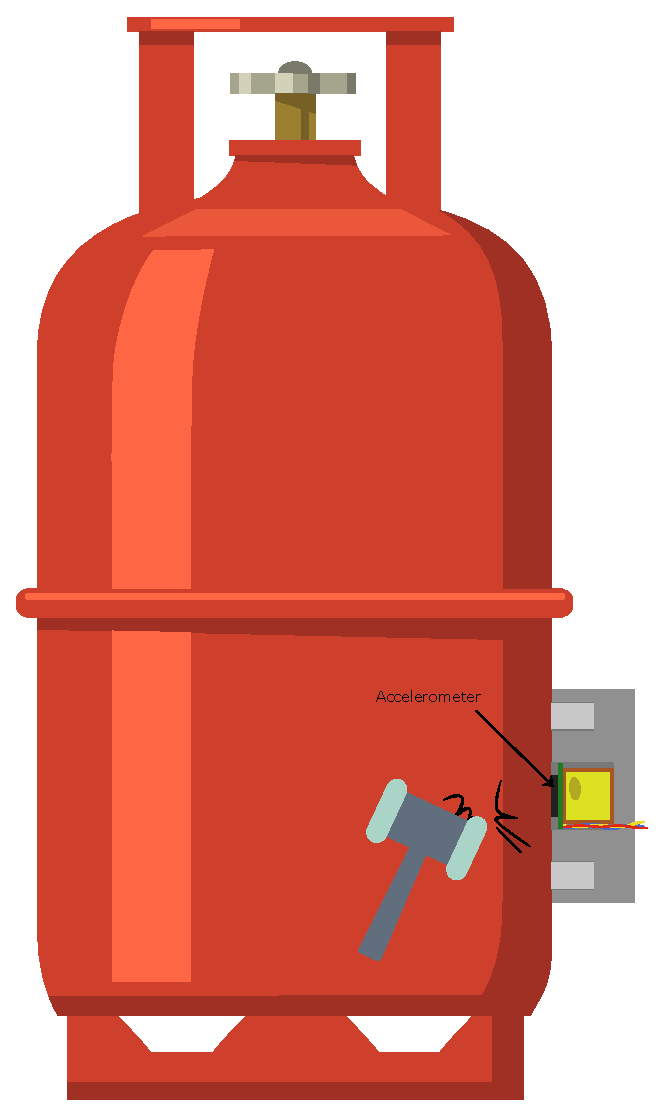
\includegraphics[width=0.3\textwidth]{Chapters/4CHP/Figures/AccMagnets.eps}
    \caption{Illustration of the accelerometer mount with magnets}
    \label{fig:mounMagnet}
\end{figure}
%

\subsection{Piezoelectric}
When mounting piezoelectric sensors, there is some considerations to take into account, those are related with the application of the sensor. \acrshort{ti} provides a document with considerations for mounting a piezoelectric sensor to measure liquid level using ultrasonic waves, although is a different approach, the key aspect for mounting this type of sensors can be used as well to define how to properly mount them. What needs to be taken into account, according to the document is, if the sensors is to be mounted inside or outside, at the top or at the bottom and for last the temperature range that the sensor can handles before starts to degrading the piezoelectric capability, it is quite clear the first aspect, since is suppose to be a non-invasive solution, which means that should be places at outside of the tank, the second aspect is not relevant since is being measured the vibration, not being used ultrasound to measure the liquid limit where the wave is reflected, the third aspect is also not that important since is expected to have the sensor at environment temperature unless, and this can be seen as an exception, when the gas from the tank has been release for a long period causing the outer wall of the bottle to freeze. Beside the first, which was already a requirement, none of the others will have a significant difference. For the purpose of measure trough the walls of the tank is required to have a good contact between the transducer and the mounting surface, in their application the glue the transducer directly to the surface of the tank \cite{minasiHowSelectMount2015}.

Since the application isn't ideal to have the transducer glued to the surface, the approach to have a good contact will be different, although the good results aren't guaranteed. The figure \ref{fig:coupPiezo} is the illustration of two different mounting pieces for the transducer.
\begin{figure}[]
    \centering
    \begin{subfigure}{0.3\textwidth}
        \centering
        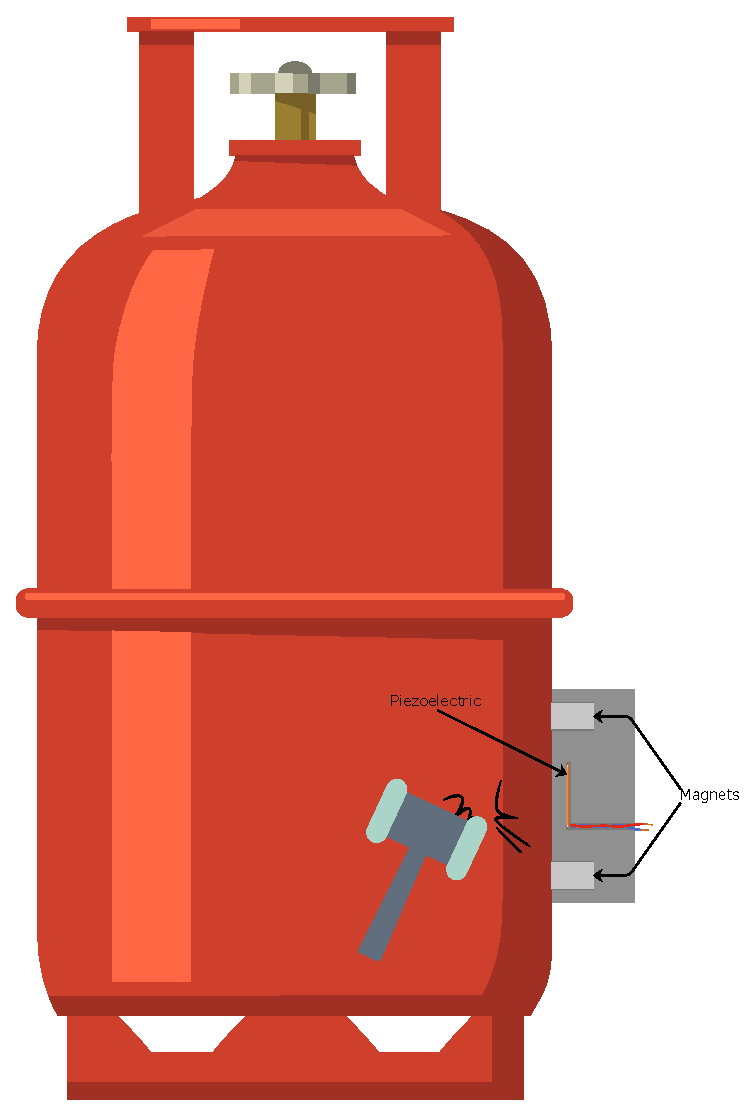
\includegraphics[width=\linewidth]{Chapters/4CHP/Figures/PiezoMagnetsSlot.eps}
        \caption{}{}
        \label{subfig:piezoslot}
    \end{subfigure}
    \begin{subfigure}{0.3\textwidth}
        \centering
        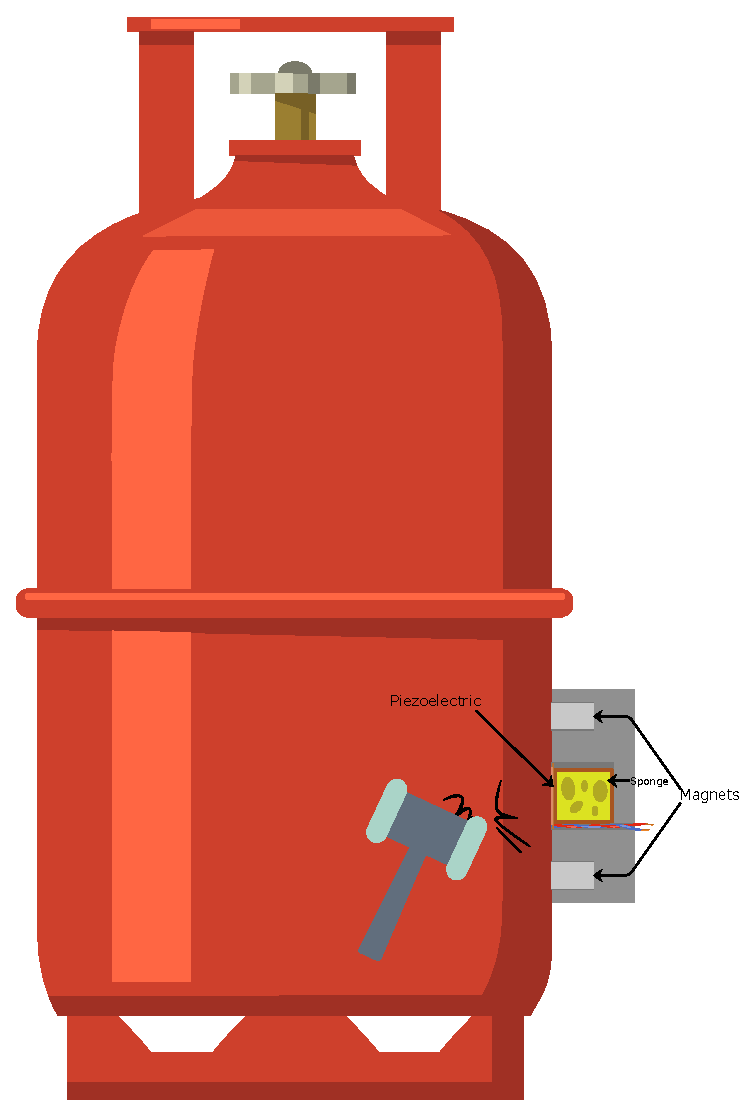
\includegraphics[width=\linewidth]{Chapters/4CHP/Figures/PiezoMagnets.eps}
        \caption{}{}
        \label{subfig:piezosponge}
    \end{subfigure}
    \caption{Illustration of the piezoelectric mount with magnets}{}
    \label{fig:coupPiezo}
\end{figure}
Both pieces will stay held to the tank with two magnets, one at the top of the piece and the other at the bottom. In figure \ref{fig:coupPiezo}~\subref{subfig:piezoslot}, the transducer is embedded in the piece, there is a slot in the middle, when the entire piece vibrates, the transducer vibrates with it. In the figure \ref{fig:coupPiezo}~\subref{subfig:piezosponge}, the coupling of the transducer is different when compared with the first one presented, the transducer is held glued to a sponge, and the sponge to the piece, the sponge is larger than the hole where the piece is glued in, so when the entire piece is attached to the walls of the tank, with the help of the magnets, it guarantees a good contact of the transducer with the wall. Since the sponge will press it against the wall and when there is vibration in the wall of the tank, is expected to the transducer to capture the actual vibration. 
\section{Extras - Delete later}
%\begin{gather}
%    \Delta_{10} = \frac{1-0}{2^{10}} \approx 0.98\cdot10^{-3}\\
%    \Delta_{8} = \frac{1-0}{2^{8}} \approx 3.9\cdot10^{-3}
%\end{gather}

%\begin{equation} \label{eq:maxf}
%    f_{Max} = \frac{1}{T-WNS} = \frac{1}{10\cdot 10^{-9} - 0.188\cdot 10^{-9}} = 101.9\,MHz
%\end{equation}

%\begin{itemize}
%    \item \textbf{AXI4} implements a highly customizable memory mapped interface, indicated for complex applications;
%    \item \textbf{AXI4-Lite} is a simplified version of the former, keeping the memory mapped communications;
%    \item \textbf{AXI4-Stream} implements a streaming protocol, allowing a high throughput.
%\end{itemize}

%\begin{figure}[!htb]
%    \centering
%    \includegraphics[width=\textwidth]{Sections/4DevelopedArchitecture/Figures/DCTCop.png}
%    \caption{Block design generated by \emph{} for integration of \emph{DCT Wrapper} with \emph{}.}
%    \label{fig:blockdes}
%\end{figure}

%\begin{table}[!htpb]
%    \centering
%    \caption{Add Caption}
%    \begin{tabular}{ccccc} \toprule
%        {}&{}&{}&{}&{}\\
%        \bottomrule
%    \end{tabular}    
    %\label{tab:maxfps}
%\end{table}


\clearpage
%\printbibliography[heading=subbibliography]
%\addcontentsline{toc}{section}{References}

%%%%%%%%%%%%%%%%%%%%%%%%%%%%%%%%%%%%%
% Developed Architecture
\cleardoublepage
\chapter{Software}
% To do: 
% Color Scheme
% Red - Not started
% Yellow - In progress
% Blue - Done, under approval
% Green - Done and approved
\todo[inline,color=red!40]{*Chapter Introduction}
\todo[inline,color=blue!40]{*1 - Microphone}
\todo[inline,color=blue!40]{ a) WOMic}
\todo[inline,color=red!40]{*2 - Accelerometer and Piezoelectric}
\todo[inline,color=red!40]{ a) Microcontroller}
\todo[inline,color=red!40]{ c) FFT implementation}
\todo[inline,color=red!40]{*3 - MatLab}
%%%%%%%%%%%%%%%%%%%%%%%%%%%%%%%%%% Writing %%%%%%%%%%%%%%%%%%%%%%%%%%%%%%%%%%%
\section{Microphone}
As the first measurements will be taken recurring to a microphone, it requires a different approach to the type of interaction when compared to the future application, were will be use a different sensor for the vibration. To obtain access and record the information from the microphone and for this case in specific, since is being used the microphone from a phone, will require different pieces of software to use in the phone side and the PC, to allow the access to the second to the microphone of the first. Also, on the PC side is necessary to record the information from the microphone and store it as desire.\\
The two components for this purpose will be the use of the WOMic software as the bridge between the phone and the computer, and MATLAB to record the information from the microphone. The second software can also be used to latter process the recorded data, helping the understand of the obtained information. 
\subsection*{WOMic}
The use of the application and the microphone of the phone is simple, although the installation and the configuration requires some time. For that, is required to install the software \textit{WOMic} in both devices, this allow to use the microphone of the phone in real-time. In the phone the software is available for Android and IOS and is responsible to transmit what is captured from the microphone, in the computer the client application and a virtual device must be installed to use the microphone in the PC to perform any type of tasks, this connection can be made over USB, Bluetooth, Wi-Fi and Wi-Fi Direct.\\ 
In order to save what is captured from the microphone, the software is split in three main block with different purposes, the \textit{WOMic App} runs in the phone, samples the input of the microphone and transmit it to the computer, the \textit{WOMic Client}, runs in the PC, connect to the app in the phone, and receive the data from the microphone, which is transmitted to the \textit{WOMic Virtual Device} on which a real microphone device is simulated and provides the audio to any application or program in the PC, as illustrated in figure \ref{fig:diagramWOMIC}.\\
\begin{figure}[!htb]
    \centering
    \includegraphics[width=0.65\textwidth]{Chapters/5CHP/Images/WOMICDiag.png}
    \caption{Flow of data in the components of the software}{\cite{WOMicFREE}}
    \label{fig:diagramWOMIC}
\end{figure}
In addition to this, is also necessary to install the drivers of the phone in use, if the connection is made over USB. To allow the access of the microphone in the PC, the transport mode must be selected on the phone application, USB in this case, in the app settings and after that start the application. In the PC the client software must be initialized and connected to the phone in the following order \textit{\>Connection\>Connect...} a new window will open, on which the USB must be selected as transport type and finalizing by pressing \textit{Connect}. With this, the microphone of the phone is available for use in the PC\cite{WOMicFREE}.
\section{Microcontroller}
%Introduction
%What is the purpose of each used element, Timer, UART, ADC, PINOUT for solenoid with timer
%What are the config of each
% Mainly from the ADC and how it works without having to use an additional timer
%
\subsection*{Timers}
\subsection*{ADC}
The LaunchPad in use offers ADC with a 10-bit, from the availabed pins, analog input 2 is selected. This input should be configured with the desire setting, to start is mandatory to disable the digital port of the pin to eliminate the flow of parasitic current flow, with the PySELx bits, by setting this bits HIGH it automatically enables the analog function of the port, although is still necessary to select the channel to conversion. The ADC will function in the sample and hold mode, using the timer from the ADC as the source of the sampling signal, the sample and hold period can be changed by software, to define the amount of clock cycles between each sample. 
\subsection*{UART}
\section{MatLab}
\section{FFT implementation}

%%%%%%%%%%%%%%%%%%%%%%%%%%%%%%%%%%%%%%%%%%%%%%%%%%%%%%%%%%%%%%%%%%%%%%%%%%%%%%

\section{??}
% \begin{figure}[!htb]
%     \centering 
%         \begin{subfigure}[c]{\textwidth}
%             \centering
%             \input{Sections/3Transforms/Images/DFTSymmetry.tex}
%             \caption{}
%             \label{subfig:dft}
%         \end{subfigure}
%         \begin{subfigure}[c]{0.45\textwidth}
%             \centering
%             \input{Sections/3Transforms/Images/DCT1Symmetry.tex}
%             \caption{}
%             \label{subfig:dct1}
%         \end{subfigure}
%         \begin{subfigure}[c]{0.45\textwidth}
%             \centering
%             \input{Sections/3Transforms/Images/DCT2Symmetry.tex}
%             \caption{}
%             \label{subfig:dct2}
%         \end{subfigure}
%         \begin{subfigure}[c]{0.45\textwidth}
%             \centering
%             \input{Sections/3Transforms/Images/DCT3Symmetry.tex}
%             \caption{}
%             \label{subfig:dct3}
%         \end{subfigure}
%         \begin{subfigure}[c]{0.45\textwidth}
%             \centering
%             \input{Sections/3Transforms/Images/DCT4Symmetry.tex}
%             \caption{}
%             \label{subfig:dct4}
%         \end{subfigure}
%         \caption{Sequences generated in the first step of Table \ref{tab:DFTDCT}for the DFT and different DCTs. Filled dots correspond to the original sequence ((a) - \emph{DFT}; (b)) - \emph{DCT-I}; (c)) - \emph{DCT-II}; (d)) - \emph{DCT-III}; (e)) - \emph{DCT-IV}).}
%     \label{fig:2NSeq}
% \end{figure}
% \begin{lstlisting}
%     ./aomenc <INPUT-FILE> -h <HEIGHT> -w <WIDTH> -o <OUTPUT-FILE> --limit=10 -p 1 --cpu-used=8 --i420 --q-hist=64 --end-usage=q --cq-level=<CQ-LEVEL>
% \end{lstlisting}
%\addcontentsline{toc}{section}{References}


%%%%%%%%%%%%%%%%%%%%%%%%%%%%%%%%%%%%%
% Developed Architecture
%\cleardoublepage
\renewcommand{\thesection}{\Alph{section}}
\begin{appendices}

%%\section{\emph{aomenc} Configuration Options} \label{app:libaom}
%%\begin{lstlisting}
%%\end{lstlisting}

%%%%%%%%%%%%%%%%%%%%%%%%%%%%%%%%%%%%%%%%%%%%%%%%%%%%%%%%%%%%%%%%%%%%%%%%%%%
%%\section{DCT8\_1 VHDL Description} \label{app:dct81}
%%\begin{lstlisting}[style=vhdl]
%%\end{lstlisting}

%%%%%%%%%%%%%%%%%%%%%%%%%%%%%%%%%%%%%%%%%%%%%%%%%%%%%%%%%%%%%%%%%%%%%%%%%%%
%%\section{DCT8\_2 VHDL Description} \label{app:dct82}
%%\begin{lstlisting}[style=vhdl]
%% \end{lstlisting}
\end{appendices}


%%%%%%%%%%%%%%%%%%%%%%%%%%%%%%%%%%%%%
% Bibliography
%\cleardoublepage
%  \nocite{*}
%  \printbibliography
%\cleardoublepage

\end{document}
